\documentclass[12pt,a4paper,openany]{book}
%------------------------------------------------------------------------------------------------------------------------------------------------------------------------------------------------------------------------------
% PACKAGES
%--------------------------------------------------------------------------------------------------------------------------------------------------------------------------------------------------------------------------------

% Selección de idioma
\usepackage[spanish]{babel}

% algo
\usepackage[utf8]{inputenc}

% Par acomodar la foto del editorial
\usepackage{wrapfig}

% Paquetes útiles
\usepackage[table]{xcolor}
\usepackage{amssymb}
\usepackage{amsmath}
%\usepackage{mathbbol}
\usepackage{bbm}
\usepackage{amsthm}
\usepackage{pdfpages}
\usepackage{graphicx,color,psfrag}
\usepackage{epstopdf}
\usepackage{pdflscape}
\usepackage{tabularx}
\usepackage{longtable}
\usepackage{breakurl}
\usepackage{enumitem}
\usepackage[normalem]{ulem}
\usepackage{blindtext}
\usepackage{mathtools,breqn}


\usepackage{fancyhdr}
\usepackage{graphicx}

\usepackage{fnpct}

\usepackage{subcaption}

\usepackage{newpxtext}
\usepackage{lscape}

% La mejor fuente de la letra: https://www3.gobiernodecanarias.org/medusa/ecoblog/lortrodm/files/2015/03/tarea-formatos-word.pdf
% caption fonts
%\usepackage[font={large,bf}]{caption} 
\usepackage[T1]{fontenc}
\usepackage{verdana}


\usepackage{setspace}
\usepackage{longtable}
\usepackage{threeparttable}  
\usepackage{tabulary}
\usepackage{booktabs}
\usepackage{float}
\usepackage{caption}
\usepackage{subcaption}
\usepackage{rotating}
\usepackage[titletoc,title]{appendix}

\usepackage{array,multirow}

\usepackage[round]{natbib}
\bibpunct{(}{)}{;}{a}{,}{;}
\setcounter{MaxMatrixCols}{10}

\topmargin=-1.8cm \textheight=23.8cm \oddsidemargin=-0.3cm
\evensidemargin=-0.5cm \textwidth=17.1cm

\newtheorem{theorem}{Theorem}
\newtheorem{corollary}[theorem]{Corollary}
\newtheorem{proposition}{Proposition}
\newtheorem{assumption}{Assumption}
\newtheorem{assumption2}{Assumption A}

\newtheorem{lemma}{Lemma}

\usepackage{tikz}
\usetikzlibrary{positioning}
\tikzset{>=stealth}
\usepackage{amsmath}
\usepackage{verbatim}
\usetikzlibrary{arrows,shapes}

% Definir colores
\definecolor{mycolor1}{RGB}{221, 165, 230}
\definecolor{mycolor2}{RGB}{54, 56, 120}	
\definecolor{mycolor3}{RGB}{205, 24, 24}
\definecolor{mycolor4}{RGB}{164, 93, 93}
\definecolor{mycolor5}{RGB}{243, 149, 13}
\definecolor{mycolor6}{RGB}{3, 83, 151}
\definecolor{mycolor7}{RGB}{52, 103, 81}
\usepackage[colorlinks=true,linkcolor=myblue, allcolors=mycolor2]{hyperref}
\usepackage{soul}

% Tablas
\usepackage{tabularx}
\usepackage{multirow}
\usepackage{multicol} 
\usepackage{booktabs}%\usepackage{booktabs, calc} %This is the package to use to have nice-looking tables. More documentation on the tables in LateX: https://www.tug.org/pracjourn/2007-1/mori/mori.pdf
\usepackage{threeparttable} 

\usepackage{lmodern}
\usepackage{booktabs}
\usepackage{pgfplots}

\graphicspath{{../figuras/}}

\begin{document}
	
	%---------------------------------------------------------------------------
	% TITLE PAGE
	%---------------------------------------------------------------------------
	\doublespacing
	
	\title{Boletín COVID-19}
	\author{Autores}
	
	\date{}

	%\maketitle
	
	
	%\thispagestyle{empty}\baselineskip1.385\baselineskip \newpage{}
	
	\pagestyle{plain}\pagenumbering{arabic}
	
	%insertar el cover
	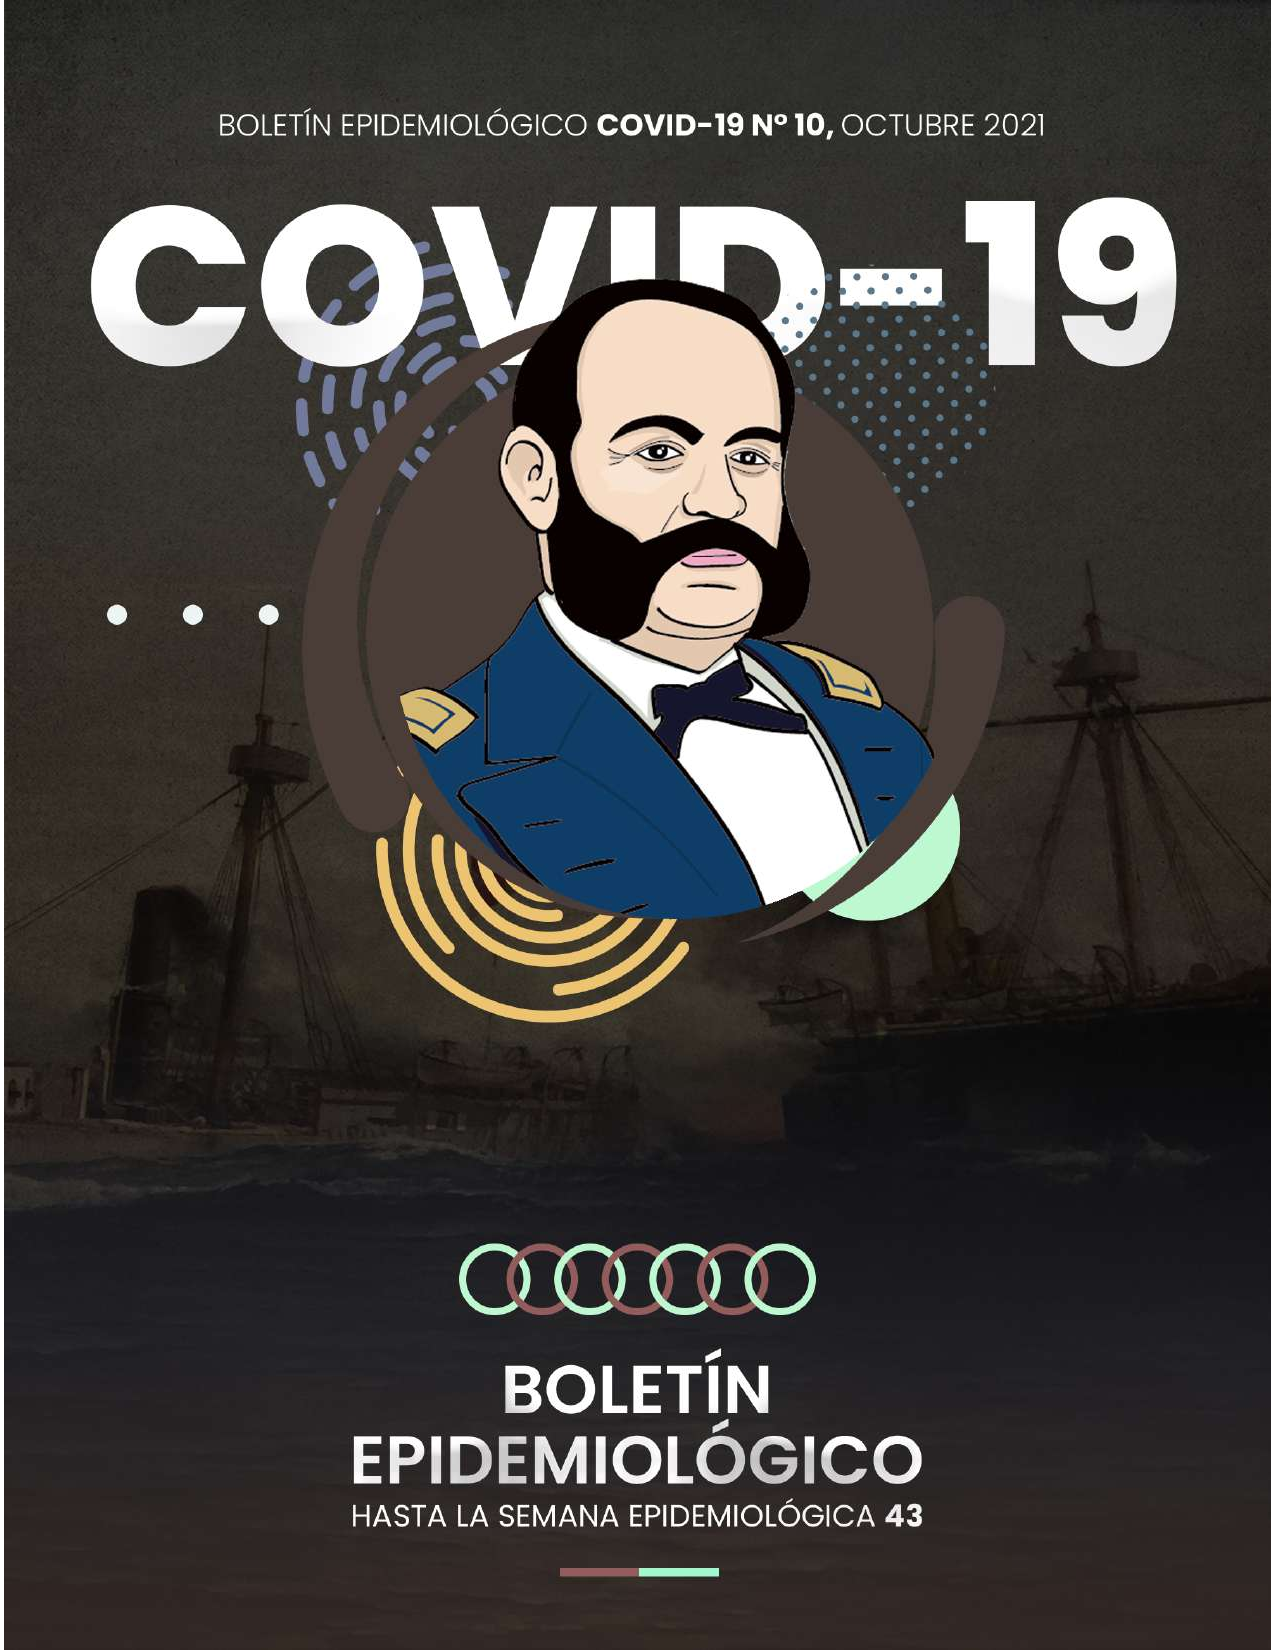
\includepdf[pages={1}]{../editorial/portada.pdf}
	\clearpage
	
	\pagestyle{plain}\pagenumbering{arabic}
	
	\clearpage
	
	
	\begin{center}
	
		{\large Gerencia Regional de Salud}
		
		\textbf{MSP. Javier Ramírez Escóbar}
		
		Gerente Regional \vspace{1.0cm}
		
		Dirección Ejecutiva de Inteligencia Sanitaria
		
		\textbf{MSP. Darío Francisco Navarro Mendoza}
		
		Director
		
		\vspace{1.5cm}
\noindent
\begin{minipage}[t]{.45\textwidth}
	\centering
	Dirección de Epidemiología e Investigación  \\
	\textbf{MSC. Fátima R. Concha Velasco}\\
	Directora \vspace{1.0cm}\\
	% Por orden alfabético del apellido
	\textit{Equipo de Epidemiología e Investigación }\vspace{.5cm}\\
	Econ. Karen Yorka Aguilar Zuñiga \\
	M.C Edwards Adrian Aguirre Valenzuela \\
	Lic. Nadia Isabel Cáceres Pillco \\
	TAP. Edgar Waldo Capcha Salcedo \\
	M.S.P. Pablo Fidel Grajeda Ancca \\
	M.C. Katia Luque Quispe \\
	M.C. Ana Gabriela Eulalia Moncada Arias \\
	Lic. Enf. Ruth Nelly Oscco Abarca \\
	Ing. Joel Wilfredo Sumerente Ayerbe \\
	Lic. Enf. Guinetta Margarita Yabar Herrera \vspace{1.5cm}\\	
\end{minipage}
\hfill
\noindent
\begin{minipage}[t]{.45\textwidth}
	\centering
	Dirección de Estadística, Informática y Telecomunicaciones\\
	\textbf{Ing. Abel Rimasca Chacón} \\
	Director \vspace{1.0cm} \\
	% Por orden alfabético del apellido
	\textit{Equipo de Estadística, Informática y Telecomunicaciones} \vspace{.5cm} \\
	Ing. Iván Atayupanqui Rondón \\
	Ing. Miguel Ángel Campana Alarcón \\
	Ing. Uriel Lacuta Farfán \\
	Ing. Jorge Fernando Lovatón Ramos \\
	Ing. Danny Robert Moscoso Sánchez \\
	Lic. Ray Milton Valderrama Álverez \vspace{1.5cm}\\
\end{minipage}
Secretaria: Sra. Ruth Baca Mendoza
	\end{center}
\let\cleardoublepage\clearpage
	\tableofcontents
\begin{center}
Visite nuestro Dashboard interactivo sobre COVID-19 haciendo clic \href{https://geresacusco.shinyapps.io/DASHBOARD\_COVID-19\_CUSCO/}{AQUÍ}
\end{center}
	
	%\mainmatter
	%---------------------------------------------------------------------------
	% CAPÍTULO: EDITORIAL
	%---------------------------------------------------------------------------

	\pagebreak
	
	\section*{Editorial}	\addcontentsline{toc}{chapter}{Editorial}
	\begin{wrapfigure}{l}{8.5cm}
		\label{wrap-fig:1}
		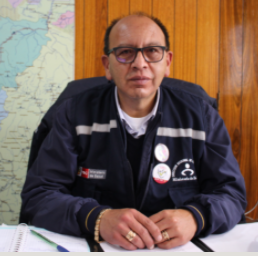
\includegraphics[width=8.5cm]{../editorial/foto_editorial_ramirez}
		\caption*{
			\centering
				MSP Cesar Javier Ramirez Escobar				
				\textit{- Gerente Regional de Salud del Cusco}
				
				 }
	\end{wrapfigure}
	
	\noindent \textbf{LOS TIEMPOS DE COVID-19 ¿LA NUEVA REALIDAD?}
 
Nuestra forma de vida apunta a que tenemos y tendremos una nueva realidad, que el coronavirus SARS-CoV-2 recorriendo el mundo nos ha cambiado y lo seguirá haciendo, que estamos haciendo y tendremos que hacer adaptaciones esenciales a nuestro estilo de vida. La humanidad se mueve entre el miedo, la incertidumbre, la readaptación a las interacciones humanas, generando agotamiento mental y diferentes estados emocionales que sin duda han provocado alteraciones biológicas y psicosociales. Se dan recomendaciones por todos lados y en todos los medios dicen cómo debe hacerse tal o cual cosa y cómo debemos comportarnos en tal o cual sitio o situación. Debido a criterios e interpretaciones, algunas indicaciones parecen asfixiantes y otras ilógicas, aunque muchas, afortunadamente la mayoría, lógicas y adecuadas y no importa que sean excesivas. Exagerar o minimizar es en esos extremos donde se mueven las opiniones y ambos hacen daño, evidentemente aun más la minimización o ignorar las medidas y no por ignorancia de conocimiento, sino con una clara idea de negar la pandemia, sus alcances y nefastas consecuencias. Se interpretan de manera estricta o laxa las cifras de contagio, de morbilidad y de fallecimientos, cada persona se vuelve experta y opina como un virólogo, epidemiólogo o estadístico poblacional, con solo un análisis apenas discreto, por decirlo de manera optimista, evidentemente sin integrar y contextualizar la opinión derivada de una información también parcial y sin contexto global. Se politiza y polariza la información y en ambos lados hay parálisis de acciones por no dar la razón a otras partes. No solo a nivel gobierno, sino en los núcleos profesionales, laborales, sociales, familiares y por supuesto en los medios de comunicación. Se critica la inacción de las estructuras de gobierno y al minuto siguiente se censura el coartar las libertades individuales por detener a un vendedor ambulante al no usar doble mascarilla y ofrecer sus productos sin las medidas de sanitarias indicadas. Se critica, con razón, la deficiente acción preventiva en aeropuertos, terminales terrestre, mercados, centros comerciales y se sale en masa para comprar sin medidas adecuadas de distanciamiento físico y uso de la doble mascarilla. Se dice que en otros países se hizo lo correcto, pero no habría disposición a toques de queda, con la participación de policía o militares para hacer cumplir el confinamiento, la aplicación de sanciones y hasta detenciones por no cumplir las disposiciones gubernamentales, tal y cómo lo han hecho países donde se aplica, se respeta y se da a respetar el estado de derecho, las autoridades, la sociedad, la comunidad y la individualidad. En nuestro país, en muchas ocasiones, la acción, la responsabilidad y el compromiso individual y comunitario es deficiente, cuando ello debería ser la base para construir una defensa efectiva ante la pandemia. ¿Nueva realidad o continuar como hasta ahora? Una sociedad con baja crítica y menor autocrítica, con baja cultura en salud y casi inexistente cultura científica. Una sociedad profundamente impregnada de interpretaciones mágico-religiosas y escaso análisis lógico-racional; que atiende rumores y dichos, aun ilógicos y muchas veces peligrosos, que desatiende medidas preventivas evidentemente correctas. Miembros de la sociedad que pueden aceptar un complot internacional, tratamientos mágicos que pueden curar todo -también la enfermedad COVID-19-, pero que no confían en el desarrollo científico de vacunas o medicamentos antivirales y menos aun de estudios serios sobre otras formas de tratamiento, que prefiere hacer caso a resultados anecdóticos y leyendas urbanas, que no tienen sistematización de resultados, ni fueron analizados con las pruebas estadísticas adecuadas. ¿Nueva realidad? Que nos lavemos las manos como deberíamos de haberlo hecho siempre y no con solo un chorro de agua y una simple pasada con el jabón, como se hacía por flojera o desidia. Lavarse las manos con frecuencia Eso se debería hacer, después de usar el transporte público, al entrar de la calle, antes de comer y después de ir al baño, muchos somos testigos de que no todos lo hacían, en el trabajo,baños,cines,restaurantes, terminales terrestres, aeropuertos. 
Sin duda debería haberse hecho siempre, no solo ahora. Usar doble mascarilla, saber estornudar con pañuelo o en la parte interna del codo, para reducir la contaminación, no salir de casa, ventilar las habitaciones, que le de luz , evitar aglomeraciones, no ir o recibir visitas cuando se tienen enfermedades respiratorias ¿Nueva realidad? No debería ser, muchas culturas lo hacen desde hace mucho, incluso el dicho de las abuelitas era que no salieras porque empeoraría la enfermedad y se podría contagiar a otros, comer bien y no exponerse a cambios de temperatura, todas las medidas que ahora parecen nuevas desde hace mucho tiempo han sido recomendaciones no solo de especialistas, sino también recomendaciones de la familia; no se hacía ¿por qué? intransigencia, inconciencia, falta de solidaridad, ignorancia, prepotencia ¿quién lo sabe? ¿Protegerse de contagios con instrumental contaminado es nuevo? ¡No! y ¿se hace algo? ¡No! ¿Cuántas personas agregan cloro o algún descontaminante a la basura, las bolsas de basura, el desecho de papel higiénico, toallas desechables? ¿Cuántos estornudan cubriéndose con la mano y enseguida usan pasamanos, perillas de puertas, platos para servir en restaurantes, utensilios de cocina y comida, alimentos crudos y procesados? Ahora calificamos como “videntes del futuro”, lo que antes eran “personas exageradas”, por ejemplo, un comensal limpiando con ahínco una botella de vino antes de abrirla y ofrecerla para su consumo o reclamando airadamente que un mesero se tocara la boca y ofreciera alguna vianda o utensilios con alimentos ¿Es ésta una nueva realidad, o debió hacerse siempre? ¿Es una nueva realidad que no se usen uniformes del personal de salud en la calle ya que con esas prendas puede contaminar y exponer a la población con esta práctica? Las batas que usan médicos y enfermeras, personal de laboratorios químicos, estudiantes de áreas biomédicas y químico-biológicas, son instrumentos de trabajo, que tienen la finalidad de proteger al paciente y al personal que la porta; el uso de la bata busca no llevar al interior la contaminación de la calle y no llevar a la calle la contaminación del área hospitalaria o del laboratorio sea biomédico o fisicoquímico. Por lo cual no se debería, ni ahora ni antes, usar batas y uniformes como un atuendo de traslado, como un uniforme escolar o laboral, porque evidentemente no lo es. Sin embargo, se podía y se puede aun ahora ver a profesionales y estudiantes comiendo fuera del área laboral con batas y uniformes de trabajo, viajando por transporte particular y público, llegando a sus casas, esperamos no sea frecuente, sin cuidar que la bata contamine su casa y a sus allegados, con mayor o menor impacto a la salud, pero siempre como un riesgo. Un apunte aparte es el estetoscopio que frecuentemente se cuelga del cuello y cuya cápsula y membrana se encontrarán a centímetros de la boca y la nariz, después de tocar el brazo, el pecho y el dorso del paciente en áreas que no fueron descontaminadas y el estetoscopio tampoco lo fue después de la auscultación ¿Será nueva realidad el manejo y portación del estetoscopio? o ¿antes no importaba y ahora sí? o ¿seguirán estas y otras prácticas una vez que en algún momento se reduzca la posibilidad de padecer COVID-19? ¿Es una nueva realidad el preocuparnos por el sobrepeso, la obesidad, la diabetes y la hipertensión, como factores de riesgo de complicaciones severas de COVID-19? No debería de serlo, las acciones de gobierno, de los sistemas de salud y sobre todo la conciencia individual deberían haber puesto en marcha o fortalecer las acciones ya iniciadas para cambiar hábitos y alimentarnos de manera sana y responsable, lo que permitiría hacer frente a otra pandemia “la obesidad” que tiene décadas avanzando contundentemente, ganando terreno y que ahora choca de lleno con esta “nueva realidad” aumentando el impacto a la salud ¿Será esta nueva realidad suficiente para ahora si tomar medidas eficientes desde el ámbito personal hasta las esferas de los programas de intervención gubernamentales? ¿O sólo se normalizará y pasará al anecdotario? En esta nueva realidad, las clases a distancia en aulas virtuales y el trabajo en casa se han tenido que implantar y desarrollar a pasos agigantados, con mayor o menor éxito, luchando con anchos de banda deficientes y mala estabilidad de las líneas de internet que tenemos en el Perú; a estas deficiencias en las tecnologías, se suma la dificultad de acceso a hardware, software y la propia experiencia de los usuarios, que no estaban, en muchos casos, ni cercanamente preparados para hacer frente de manera eficiente al reto planteado. Lo anterior, aunado a las dificultades para que los alumnos cuenten con los dispositivos que les permitan generar una comunicación adecuada, ahora transferida al ámbito digital, Los tiempos de COVID-19 , la falta de contacto visual, la dificultad para usar la expresión corporal, la concentración de los alumnos y profesores, la posibilidad de instalarse en una reunión, conectarse a la reunión y realizar otras actividades y la salida de las reuniones por caída de la red informática, entre otras dificultades. Aun con el desarrollo impresionante de plataformas de comunicación a distancia muchas instituciones han quedado rezagadas en el desarrollo y promoción de tales herramientas, la generación de firmas digitales, la adaptación de aulas virtuales para el desarrollo de reuniones mixtas de manera cotidiana. En tal sentido la pandemia no generará otra realidad, nos llevará obligadamente a una realidad a la que nos resistíamos a entrar. Dentro de la incertidumbre vamos avanzando para entender qué y cómo será esa supuesta nueva realidad. Esperemos que nos lleve a un mejor estado en los diferentes aspectos, que no se diluyan las buenas prácticas, regresemos al mismo lugar y que sepamos afrontar las cosas difíciles, adaptándolas, integrándolas y que de todo esto resulte algo mejor en todos los aspectos posibles.

	
	
	%---------------------------------------------------------------------------
	% CAPÍTULO: METODOLOGÍA
	%---------------------------------------------------------------------------
			%insertar el cover del capitulo
	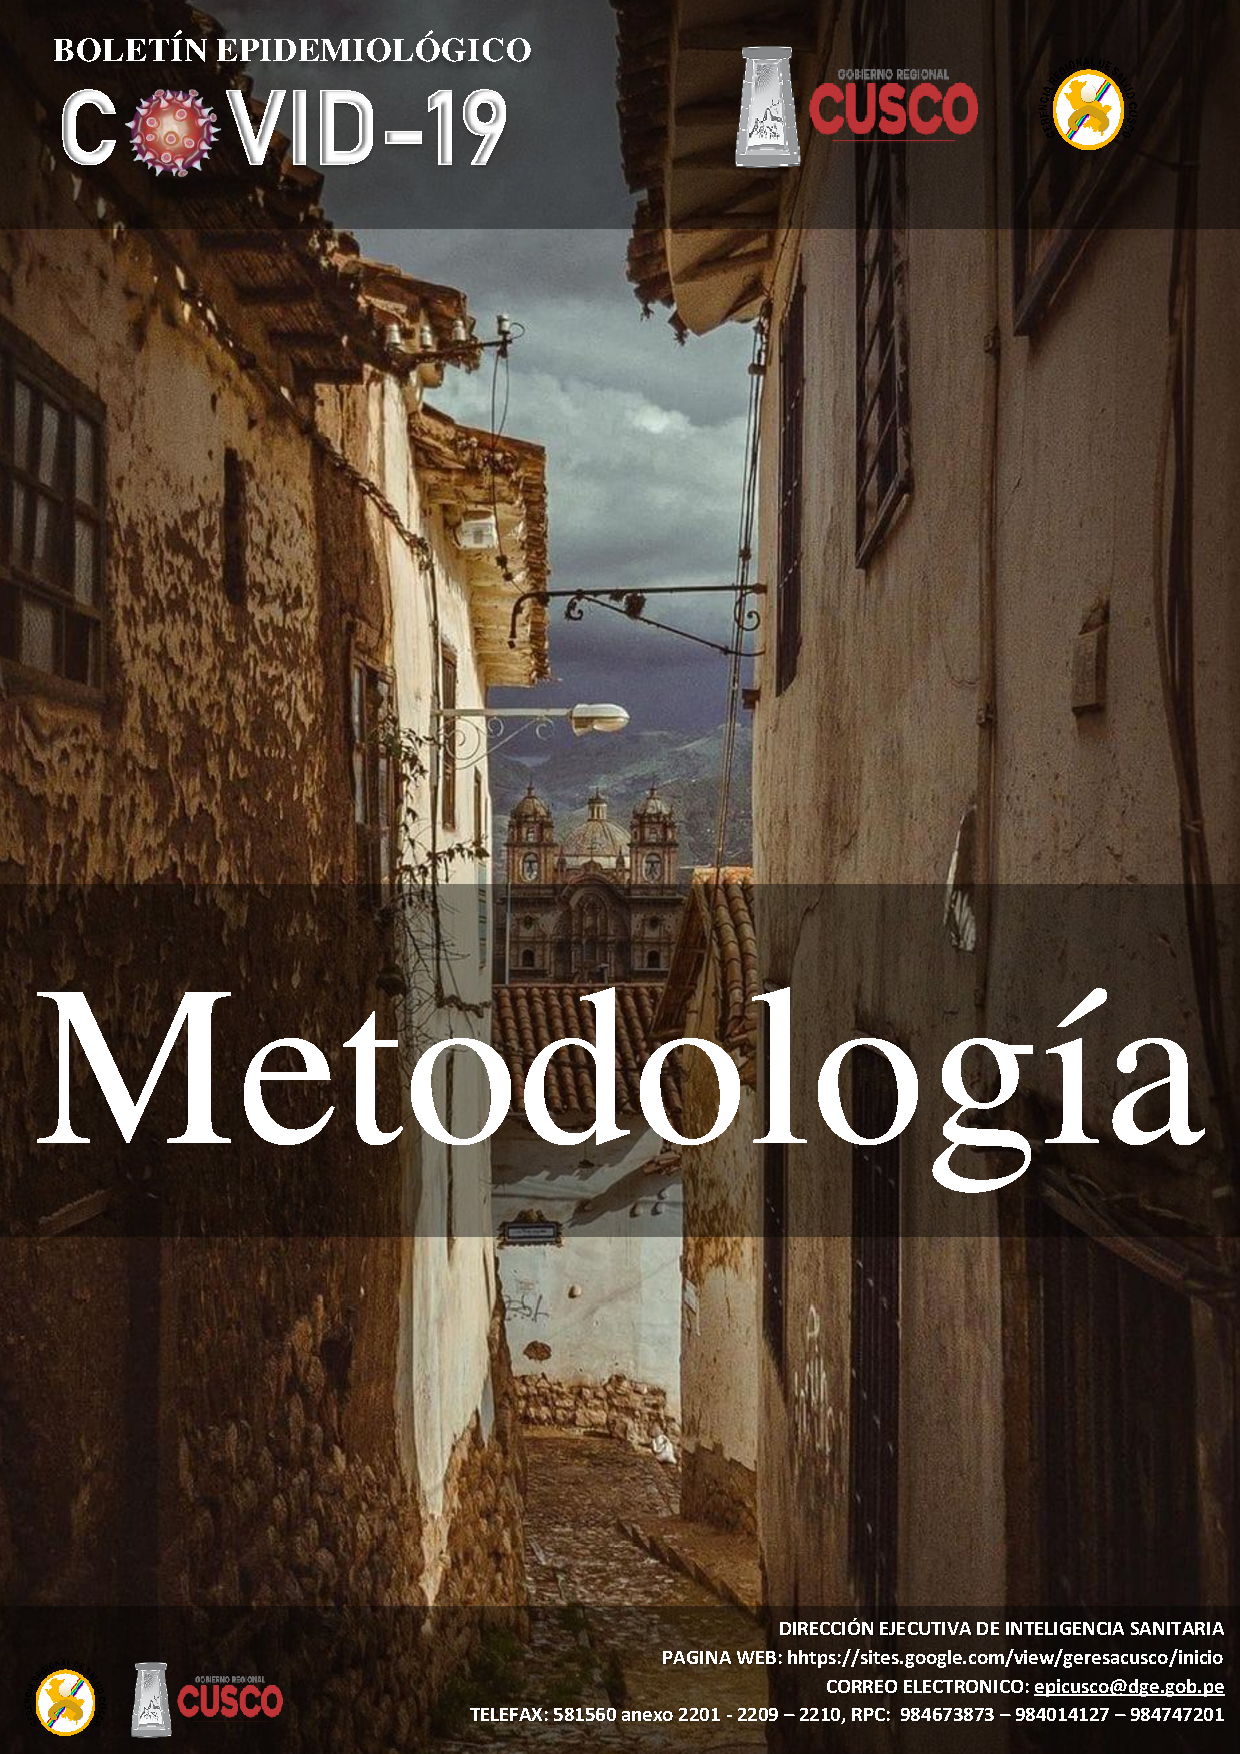
\includepdf[pages={1}]{../editorial/1.pdf}
	\clearpage
	
	\section*{Metodología}	
	\addcontentsline{toc}{chapter}{Metodología}
	\noindent El presente Boletín tiene el objetivo de informar sobre los principales indicadores epidemiológicos y de gestión hospitalaria,  para hacer el seguimiento de la pandemia en nuestra región y tomar mejores decisiones. Este Boletín tiene una metodología de tipo descriptiva. 
	
	En él, se encuentra un análisis extensivo de la situación actual de la pandemia en nuestra región desde la semana epidemiológica (SE) 1 a la 51 del 2021 (3 de enero al 25 de diciembre del 2021).
	
	Los datos analizados incluyeron: a) características generales: sexo, edad, casos confirmados, fallecidos; b) características clínicas: síntomas reportados, casos confirmados sintomáticos, casos confirmados asintomáticos y comorbilidades; c) indicadores epidemiológicos: sistema de vigilancia epidemiológica, tasa de mortalidad, tasa de positividad de pruebas diagnósticas, casos activos – recuperados, y exceso de muerte por todas las causas, y d) indicadores de gestión hospitalaria: , ocupación de camas UCI y No UCI en la Región. En este boletín se considera como caso positivo de Covid-19, sólo a aquellos que tienen una prueba antigénica o molecular positiva, salvo en ciertas estimaciones, en cuya descripción se detalla si se utilizó otro tipo de examén diagnóstico. 
	
	Las fuentes de información son las bases de datos de NOTI WEB (aplicativo del Sistema de Vigilancia Epidemiológica - COVID-19), SISCOVID (Sistema Integrado para COVID-19), SINADEF (Sistema Informático Nacional de Defunciones), SICOVAC-HIS MINSA(Base de datos de vacunación por COVID-19), Reporte de Disponibilidad de Camas de Hospitalización y datos de la Oficina de Referencias-Contrarreferencias de la Dirección de Emergencias y Desastres de GERESA-Cusco. 
	
	Se usaron frecuencias absolutas y relativas para la descripción de los datos cualitativos. Para la descripción de datos cuantitativos se calcularon tasas (mortalidad, pruebas diagnósticas, incidencia de casos), promedios (ocupación de camas hospitalarias, fallecidos por COVID y fallecidos por todas las causas). Para describir la tendencia se representaron los datos cuantitativos y frecuencias relativas en intervalos de 7 días (semana epidemiológica). En las variables de sistema de vigilancia epidemiológica (1 prueba por 100,000 habitantes) y ocupación de cama (adecuado, menor a $70\%$, moderado, entre $75$ a $90\%$ y limitado, más de $90\%$), siendo todos los puntos de referencia sugeridos por la Organización Mundial de la Salud. Para el análisis de exceso de mortalidad, se usó la metodología descrita por C. Giattino, H. Ritchie, M. Roser, E. Ortiz-Ospina, y J. Hasell en el artículo "Excess mortality during the Coronavirus pandemic (COVID-19)". Published online at OurWorldInData.org.
	
	La descripción de dichas variables se hace de manera regional y provincial. En la presente edición se hace una descripción de la tasa de incidencia, tasa de mortalidad, tasa de positividad por prueba molecular y antigénica, y exceso de defunciones de todas las provincias de nuestra región. El lector interesado en un análisis distrital de los casos y defunciones puede encontrar en los links correspondientes.
	 
	%---------------------------------------------------------------------------
	% CAPÍTULO: CARACTERÍSTICAS GENERALES
	%---------------------------------------------------------------------------
		%insertar el cover del capitulo
	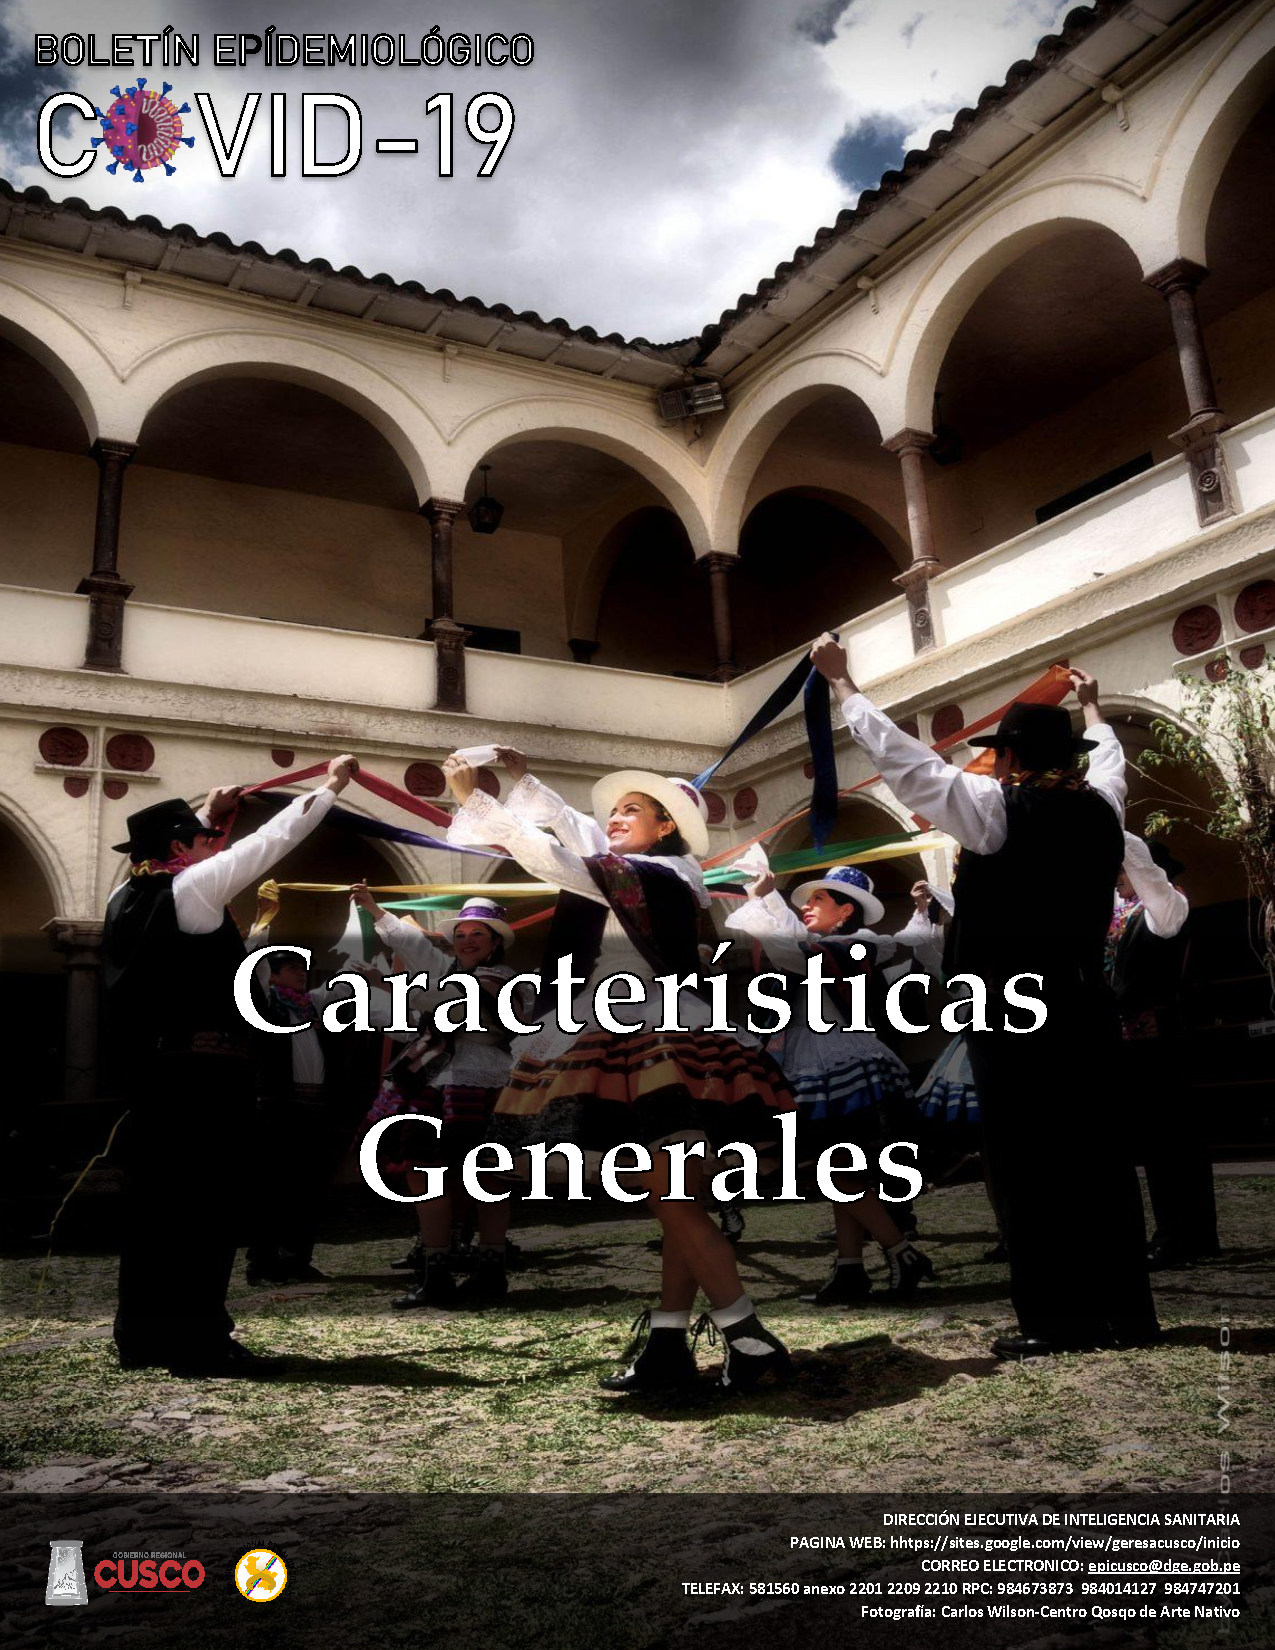
\includepdf[pages={1}]{../editorial/2.pdf}
	\clearpage	
	\section*{Características Generales}
	\addcontentsline{toc}{chapter}{Características Generales}
	
	
	
 	\noindent En la Figura \ref{fig:casos_edad_sexo} se muestra la cantidad de casos confirmados de COVID-19, por prueba antigénica o molecular, hasta la SE 51 por grupo etario (en intervalos de 10 años) y sexo. La mayor cantidad de casos se concentra en los grupos etarios de 30 a 39 años, con un total de 11 041 casos acumulados, seguido del grupo etario de 20 a 29 años, con un total de 9 733. Según la distribución por sexo, la cantidad de mujeres superó a los varones en los grupos etarios de 10 a 40 años, en el resto de grupos la diferencia de casos entre ambos sexos es reducida.  
 	
 	
 	
	\begin{figure}[h]
		\caption{Casos Confirmados de COVID-19 según Grupo de Edad y Sexo en la Región Cusco, hasta la SE 51.}\label{fig:casos_edad_sexo}
		\begin{center}
			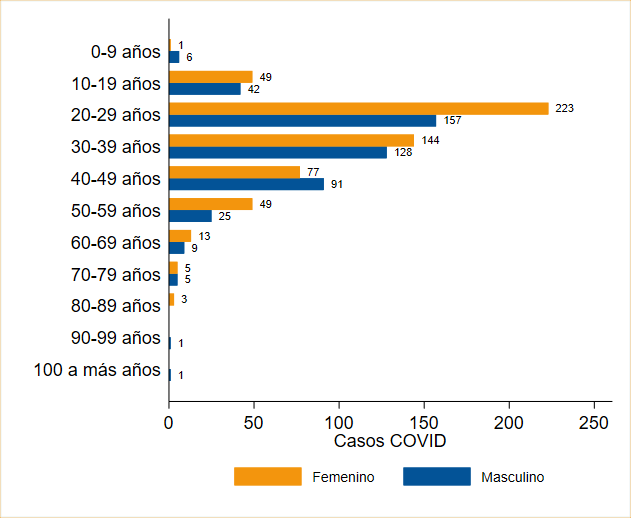
\includegraphics[width=0.75\linewidth]{../figuras/casos_etapavida}
		\end{center}
		{\footnotesize {Fuente de datos: SISCOVID, NOTICOVID.}}
	\end{figure}
\pagebreak

La Figura  \ref{fig:fallecidos_edad_sexo}  muestra el número de muertes debido a COVID-19 por grupo etario y sexo. Se puede apreciar que el mayor número de muertes se reporta en el grupo etario de 70 a 79 años(780 muertes acumuladas), seguido del grupo etario de 60 a 69 años (713 muertes acumuladas). La cantidad de fallecidos en el sexo masculino supera a la cantidad de fallecidos de sexo femenino.
	\begin{figure}[h]
		\caption{Casos fallecidos por COVID-19 según Grupo Etario y Sexo en la Región Cusco, hasta la SE 51, 2021.}\label{fig:fallecidos_edad_sexo}
		\begin{center}
			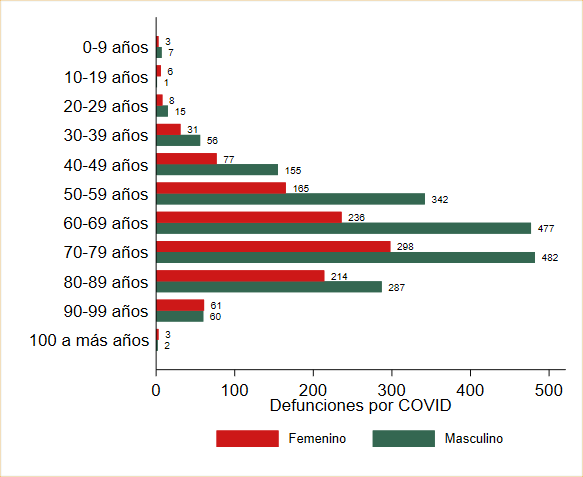
\includegraphics[width=0.75\linewidth]{../figuras/defunciones_etapavida}
		\end{center}
		{\footnotesize {Fuente de datos: SISCOVID, NOTICOVID.}}
	\end{figure}


\cleardoublepage
%---------------------------------------------------------------------------
% CAPÍTULO: CARACTERÍSTICAS CLÍNICAS
%---------------------------------------------------------------------------
	%insertar el cover del capitulo
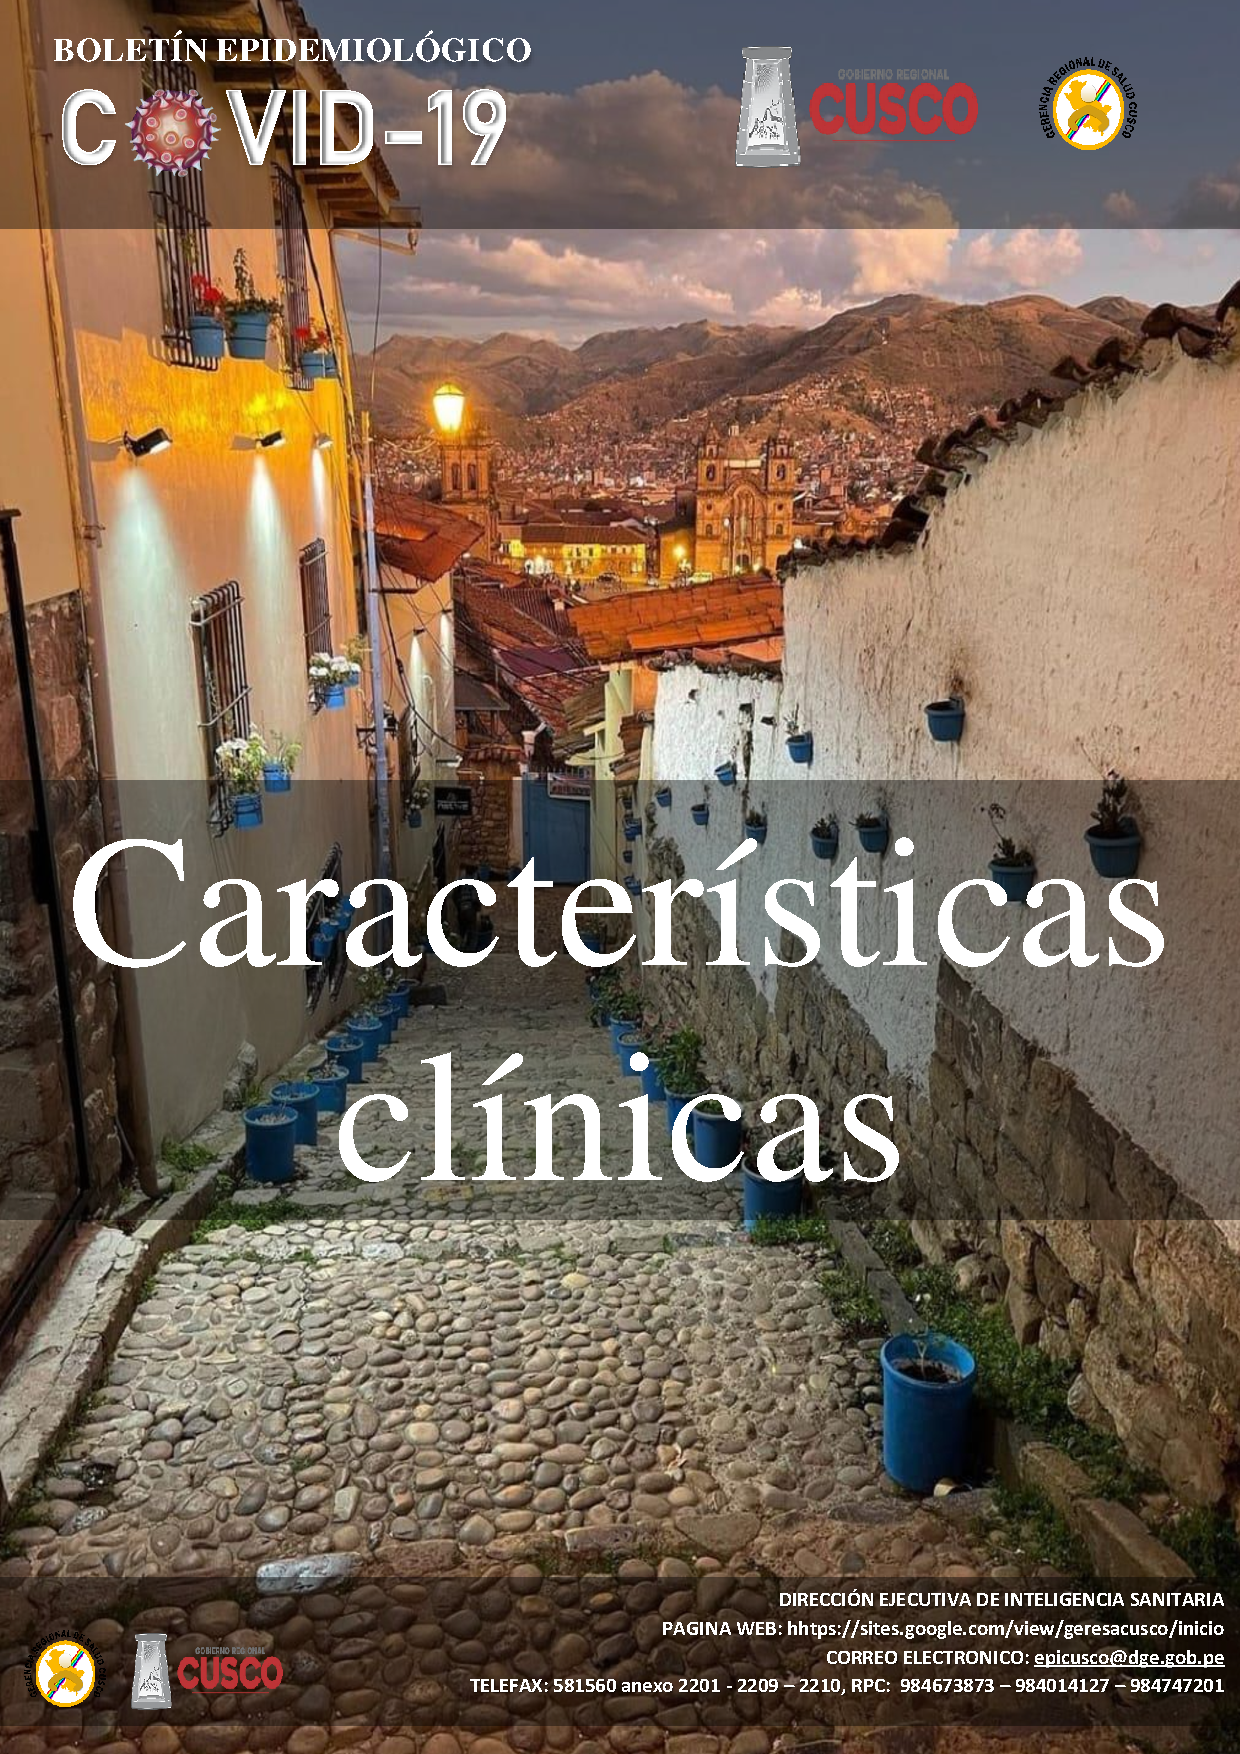
\includepdf[pages={1}]{../editorial/3.pdf}

\clearpage

\section*{Características Clínicas}
\addcontentsline{toc}{chapter}{Características Clínicas}	


\noindent En la Figura \ref{fig:sintomas}, se presentan los síntomas más frecuentes de los pacientes diagnosticados con COVID-19, el síntomas más frecuente es la tos (15,1$\%$), seguido de dolor de garganta (14,4$\%$). Con respecto a los signos clínicos, en la Figura \ref{fig:signos} se evidencia que el exudado faríngeo (63,8$\%$) es el signo más frecuente. 

\begin{figure}[h]
	\caption{Síntomas más frecuentes de los pacientes diagnosticados por COVID-19 en la Región Cusco, hasta la SE 51, 2021.  }\label{fig:sintomas}
	\begin{center}
		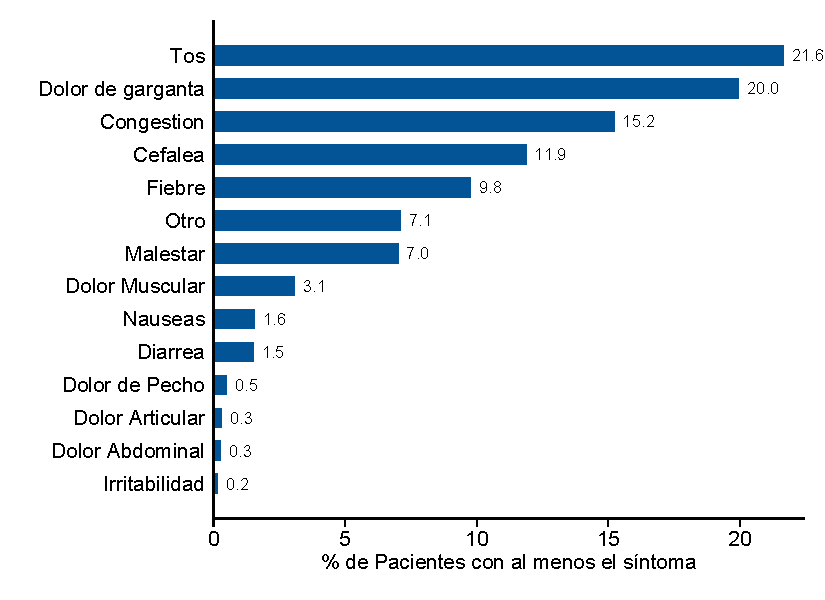
\includegraphics[width=0.85\linewidth]{../figuras/figura_sintoma.pdf}
	\end{center}
	{\footnotesize {Fuente de datos: SISCOVID, NOTICOVID.}}
\end{figure}

\begin{figure}[h]
	\caption{Signos más frecuentes de los pacientes diagnosticados por COVID-19 en la Región Cusco, hasta la SE 51, 2021.}\label{fig:signos}
	\begin{center}
		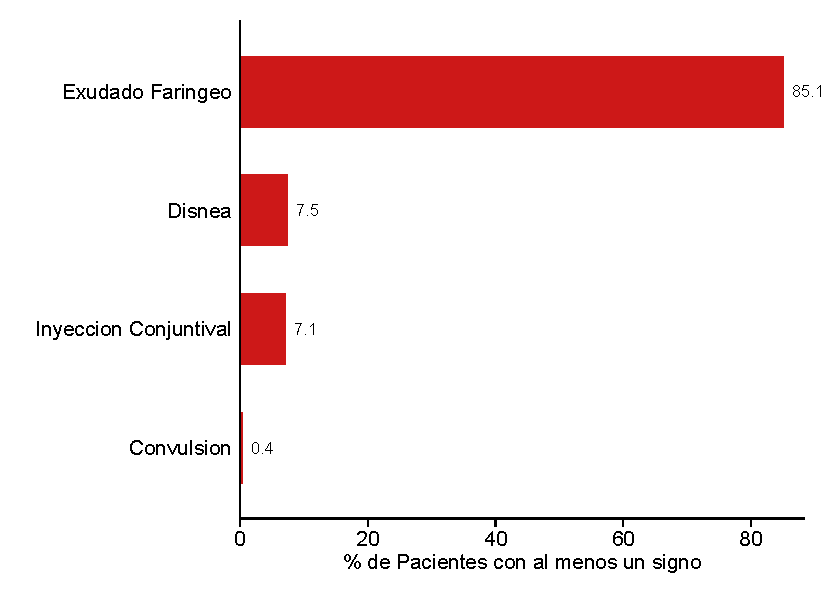
\includegraphics[width=0.65\linewidth]{../figuras/figura_signo.pdf}
	\end{center}
	{\footnotesize {Fuente de datos: NOTICOVID.}}
\end{figure}

La comorbilidades más frecuentes se encuentran graficadas en la Figura \ref{fig:comorbilidades}. La obesidad es la comorbilidad más frecuente con una prevalencia de 26,4$\%$, seguido de Diabetes con 22,0$\%$. 
\begin{figure}[h]
	\caption{Comorbilidades más frecuentes de los pacientes diagnosticados por COVID-19 en la Región Cusco, hasta la SE 51, 2021. }\label{fig:comorbilidades}
	\begin{center}
		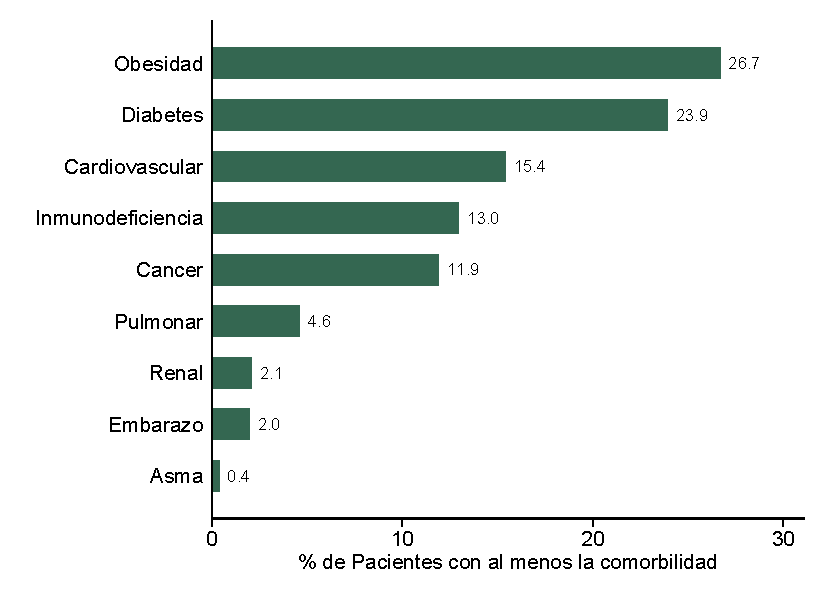
\includegraphics[width=0.65\linewidth]{../figuras/figura_comorbilidad.pdf}
	\end{center}
	{\footnotesize {Fuente de datos: NOTICOVID.}}
\end{figure}
\clearpage
 En la Figura \ref{fig:sintomaticos_asintomati} se evidencia la curva epidémica de casos sintomáticos y asintomáticos detectados por pruebas moleculares, antigénicas o pruebas rápidas, comparada con los casos sintomáticos y asintomáticos del 2020. Para el año 2021, se evidencia que hubo un incremento discreto de casos asintomáticos en la SE 43 y su posterior descenso para la SE 46. Con respecto a los casos sintomáticos, la tendencia se mantiene sin cambios marcados desde la SE 29. 
 
 
\begin{figure}[h]
	\caption{Casos Sintomáticos y Asintomáticos de COVID-19, por Semana Epidemiológica en la Región Cusco, hasta la SE 51,2021.  }\label{fig:sintomaticos_asintomati}
	
	\begin{center}
		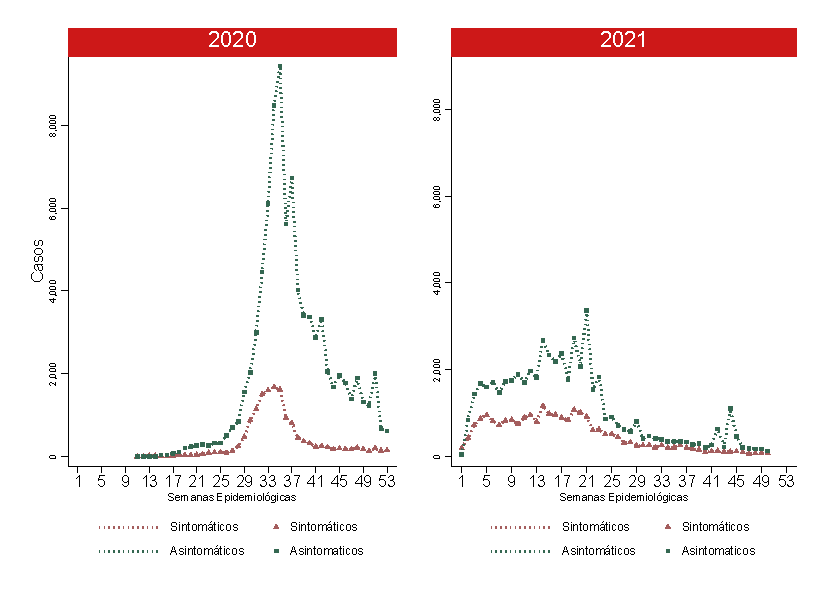
\includegraphics[width=0.75\linewidth]{../figuras/sintomaticos_20_21.pdf}
	\end{center}
	{\footnotesize {Fuente de datos: SISCOVID, NOTICOVID.}}
\end{figure}
\clearpage

%---------------------------------------------------------------------------
% CAPÍTULO: ANÁLISIS DE INDICADORES
%---------------------------------------------------------------------------
%insertar el cover del capitulo
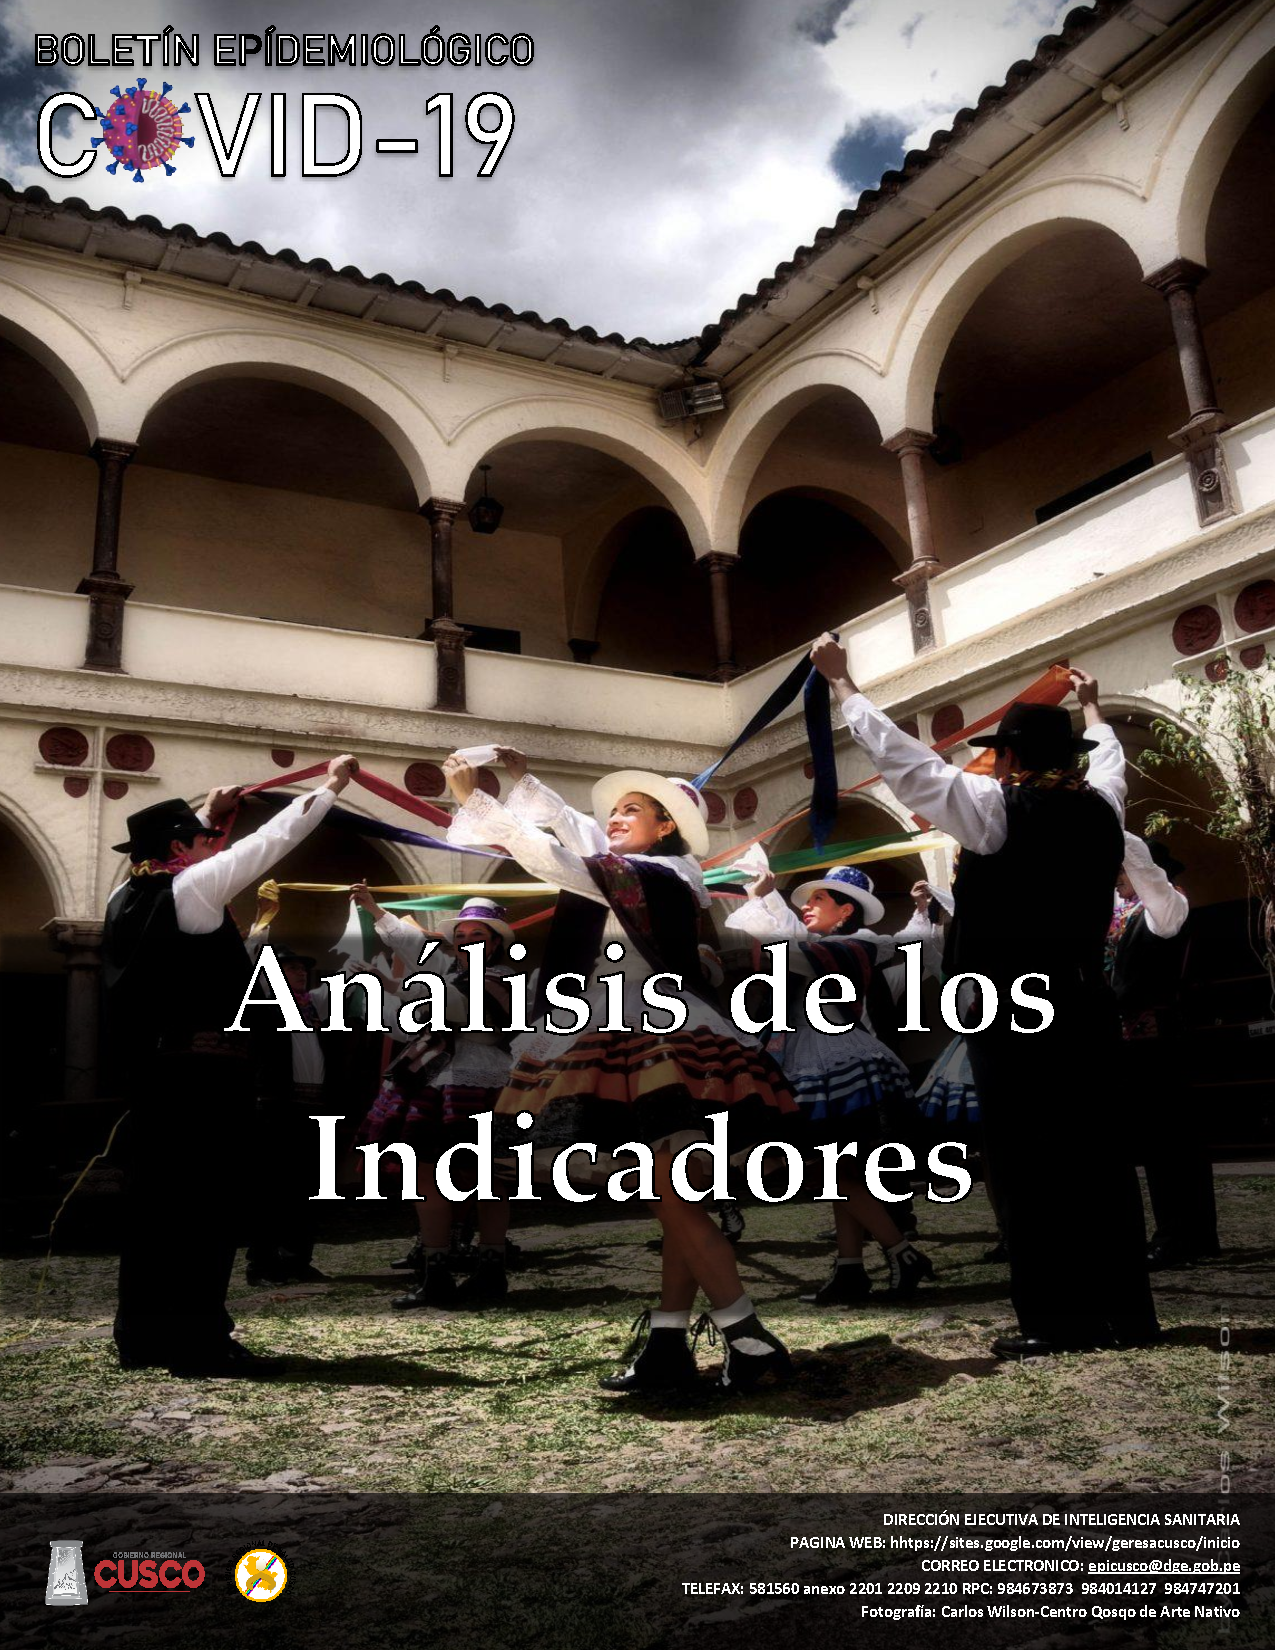
\includepdf[pages={1}]{../editorial/4.pdf}
\clearpage

    \section*{Análisis de Indicadores}
    \addcontentsline{toc}{chapter}{Análisis de Indicadores}
   	\subsection*{Tasa de Incidencia y Tasa de Positividad}
\noindent La evolución de la tasa de incidencia en el tiempo se encuentra graficada en la Figura \ref{fig:incidencia}, desde la SE 45, la tasa de indicencia presentó un descenso durante 6 semanas consecutivas hasta la SE 51,  donde presenta un discreto incremento con respecto a la semana previa. En la última semana la tasa de incidencia fue de 14 casos/ 1 000 000 personas.  

   \begin{figure}[h]
   	\caption{Tasa de Incidencia de COVID-19 en la región Cusco hasta la SE 51*. }\label{fig:incidencia}
   	\begin{center}
   		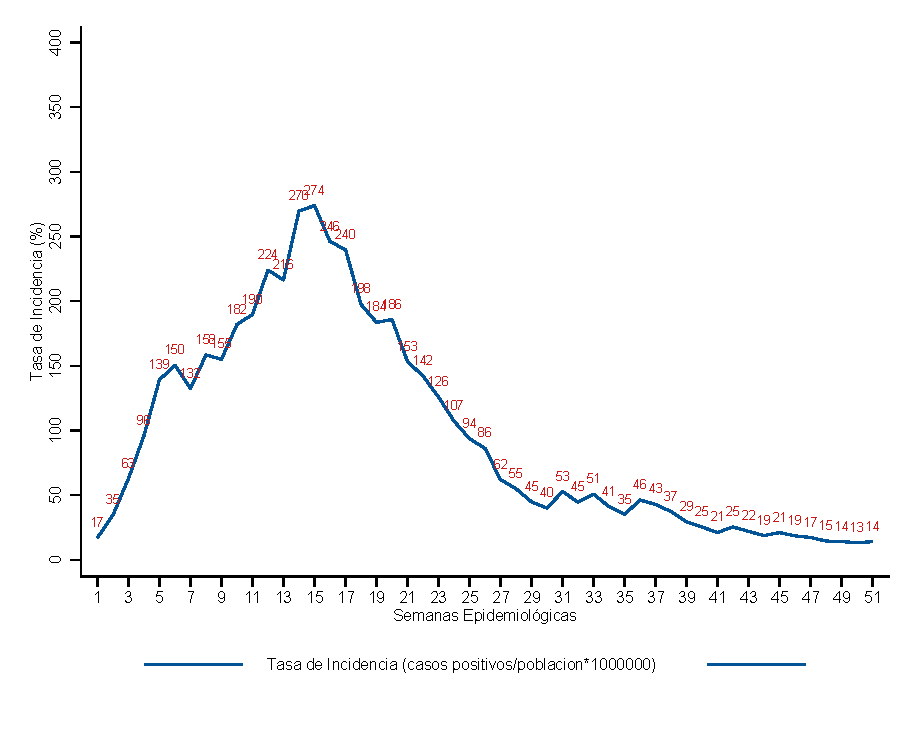
\includegraphics[width=0.85\linewidth]{../figuras/tasa_incidencia.pdf}
   	\end{center}
   	{\footnotesize {Fuente de datos: SISCOVID, NOTICOVID. (*) Se considera como caso positivo sólo a los pacientes con prueba molecular o antigénica positiva.}}
   \end{figure}
   
   La Figura \ref{fig:total_muestras_procesada} muestra un comparativo de las Tasas de Positividad ($\%$) de pruebas moleculares(PCR) y antigénicas(AG). El pico máximo de la tasa de positividad de pruebas moleculares se presentó en la SE 11, tras los cual se observó un descenso gradual hasta la fecha.
   
   Mientras que la tasa de positividad de pruebas antigénicas tuvo su pico máximo en la SE 14, tras lo cual tuvo un descenso sostenido hasta la fecha.
  
   
   \begin{figure}[h]
   	\caption{Tasa de positividad para muestras antigénicas y moleculares por COVID-19 en la región Cusco hasta la SE 51. }\label{fig:total_muestras_procesada}
   	\begin{center}
   		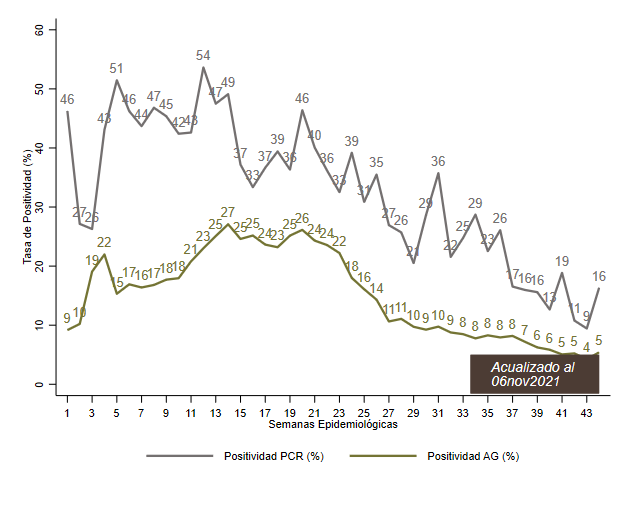
\includegraphics[width=0.80\linewidth]{../figuras/positividad_diaria}
   	\end{center}
   	{\footnotesize {Fuente de datos: SISCOVID, NOTICOVID.}}
   \end{figure}



La Figura \ref{fig:positividad_ambas} muestra el comparativo de las tasas de positividad y el número de pruebas positivas antigénicas y moleculares. Se muestra en ambos casos un descenso sostenido de la tasa de positividad de pruebas moleculares y antigénicas hasta la fecha. 
\begin{landscape}
   \begin{figure}[h]
	\caption{Positividad y Tasa de Positividad de pruebas moleculares y antigénicas tomadas por COVID-19 en la región Cusco, hasta la SE 51.}\label{fig:positividad_ambas}
   	\begin{center}
   		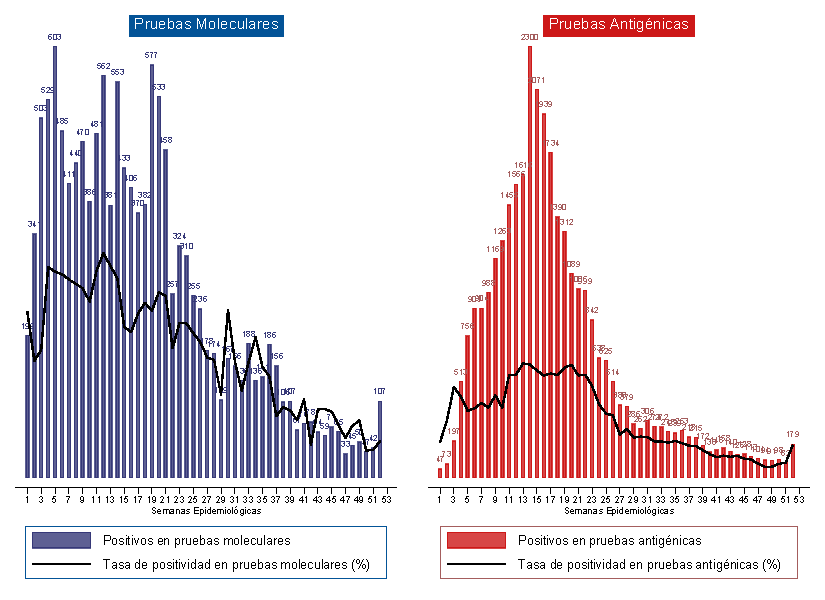
\includegraphics[width=0.85\linewidth]{../figuras/positividad_ambas.pdf}
   	\end{center}
   	{\footnotesize {Fuente de datos: SISCOVID, NOTICOVID.}}
   \end{figure}
\end{landscape}
\clearpage

	\subsection*{Análisis de la Mortalidad}

	\noindent En la Figura \ref{fig:mortalidad_edad} muestra la mortalidad semanal para las edades agrupadas en diez años. Desde la SE 25, la tasa de mortalidad de todos los grupos etarios ha mostrado una marcada pendiente al descenso. El grupo etario de 80 años a más, presenta la tasa de mortalidad más alta, sin embargo desde la SE 50 no se reportaron muertes por COVID-19 en este grupo etario. 	
	\begin{figure}[h]
	\caption{Tasa de Mortalidad por COVID-19 por Grupo Etario, hasta la SE 51.}\label{fig:mortalidad_edad}
	\begin{center}
		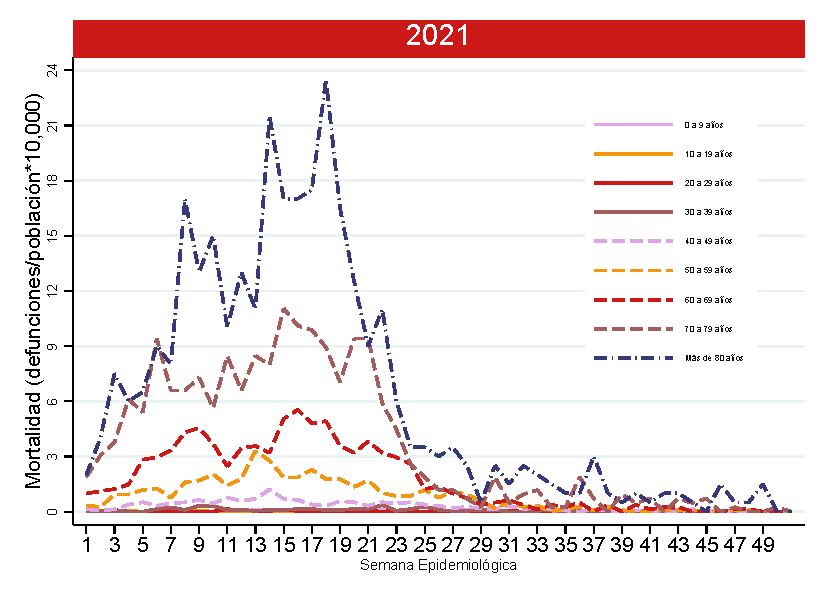
\includegraphics[width=0.65\linewidth]{../figuras/mortalidad_edad.pdf}
	\end{center}
	{\footnotesize Fuente de datos: SINADEF} 
	\end{figure}


	La Figura \ref{fig:mortalidad_grupo_edad} muestra la relación entre la tasa de mortalidad y la vacunación. Las líneas de referencia representan las fechas del inicio de la vacunación (primera y segunda dosis) para el correspondiente grupo etario. 
	
	Se observa que tras la administración de dos dosis de vacuna contra COVID-19,  hay una pendiente marcada en descenso de la tasa de mortalidad. 

	\begin{figure}[h]
	\caption{Tasa de Mortalidad por COVID-19 por Grupo Etario, hasta la SE 51.}
	\label{fig:mortalidad_grupo_edad}
	\centering
	\begin{subfigure}[b]{0.45\textwidth}
		\centering
		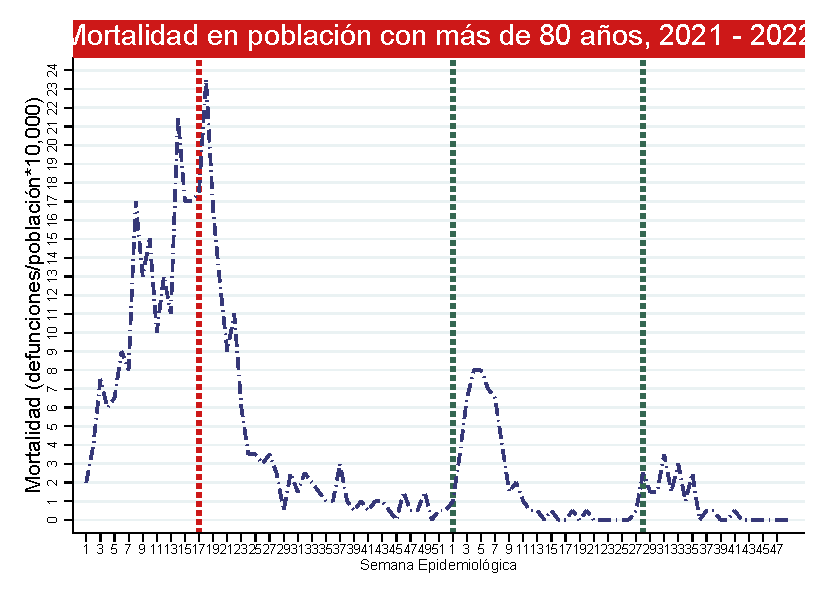
\includegraphics[width=\textwidth]{../figuras/mortalidad_edad_80.pdf}
		\caption{Más de 80 años}
		%\label{fig:}
	\end{subfigure}
	\hfill
	\begin{subfigure}[b]{0.45\textwidth}
		\centering
		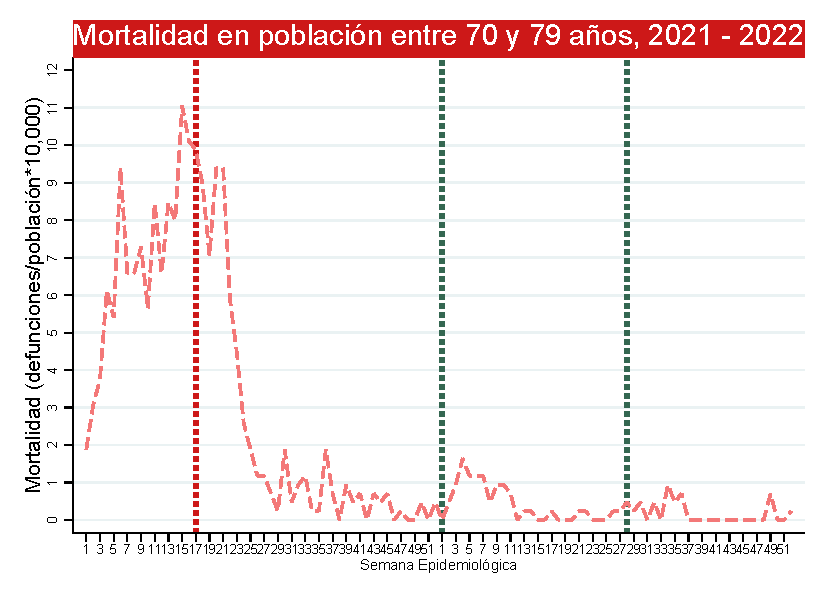
\includegraphics[width=\textwidth]{../figuras/mortalidad_edad_70.pdf}
		\caption{70 a 79 años}
		%\label{fig:70 a 79 años}
	\end{subfigure}

	\vspace{10mm}
	\begin{subfigure}[b]{0.45\textwidth}
		\centering
		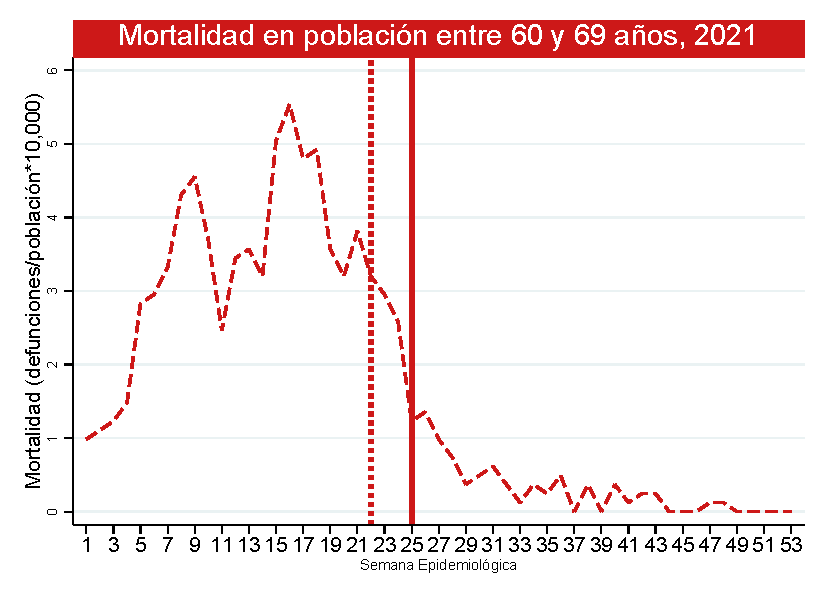
\includegraphics[width=\textwidth]{../figuras/mortalidad_edad_60.pdf}
		\caption{60 a 69 años}
		%\label{fig:60 a 69 años}
	\end{subfigure}
	\hfill
	\begin{subfigure}[b]{0.45\textwidth}
		\centering
		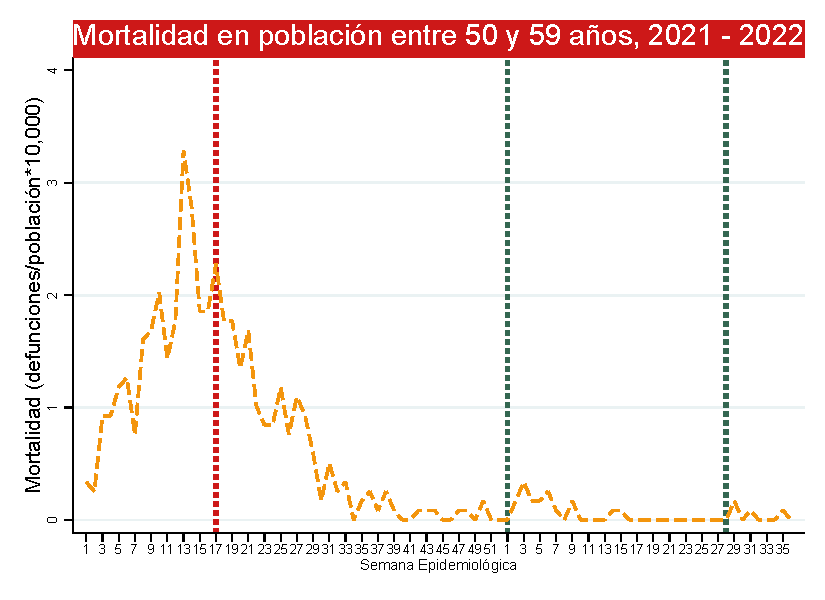
\includegraphics[width=\textwidth]{../figuras/mortalidad_edad_50.pdf}
		\caption{50 a 59 años}
		%\label{fig:50 a 59 años}
	\end{subfigure}

	\vspace{10mm}
	\begin{subfigure}[b]{0.45\textwidth}
		\centering
		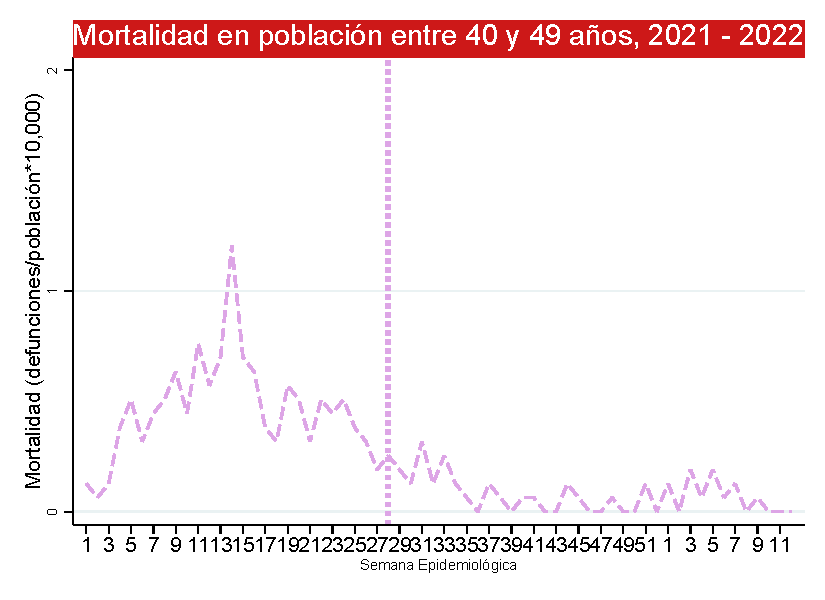
\includegraphics[width=\textwidth]{../figuras/mortalidad_edad_40.pdf}
		\caption{40 a 49 años}
		%\label{fig:40 a 49 años}
	\end{subfigure}
	\hfill
	\begin{subfigure}[b]{0.45\textwidth}
		\centering
		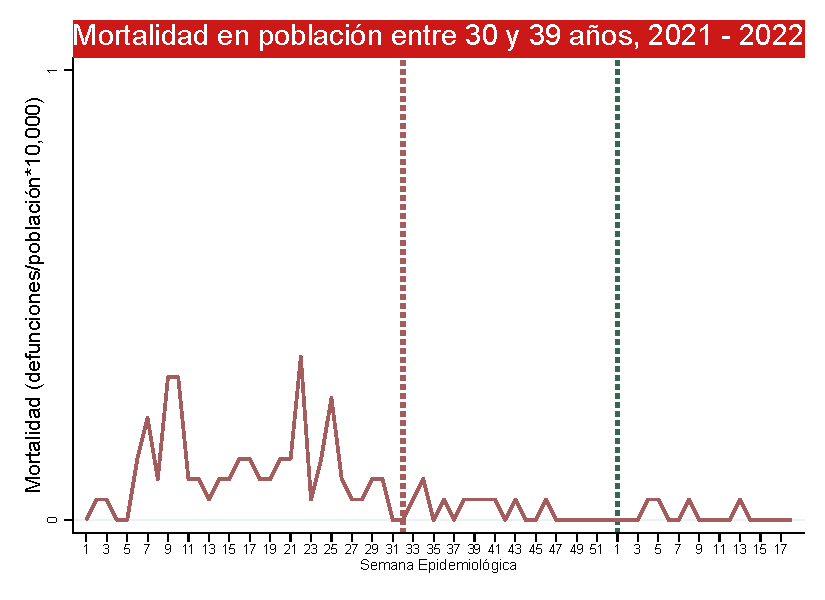
\includegraphics[width=\textwidth]{../figuras/mortalidad_edad_30.pdf}
		\caption{30 a 39 años}
		%\label{fig:40 a 49 años}
	\end{subfigure}
	\end{figure}

\clearpage
2	
	\subsection*{Exceso de Muertes por Todas las Causas}
	\noindent  La Figura \ref{fig:exceso_regional} muestra la tendencia del exceso de muertes con respecto al año 2019. Para la SE 51, el exceso de muertes en el año 2021 presentó una pendiente en descenso comparada con respecto al año 2019, lo que se traduce en un exceso de muerte negativo (menos 16). 

	\begin{figure}[h]
	\caption{Exceso de Fallecidos por Todas las Causas en la Región Cusco,  hasta la SE 51.}\label{fig:exceso_regional}
	\begin{center}
		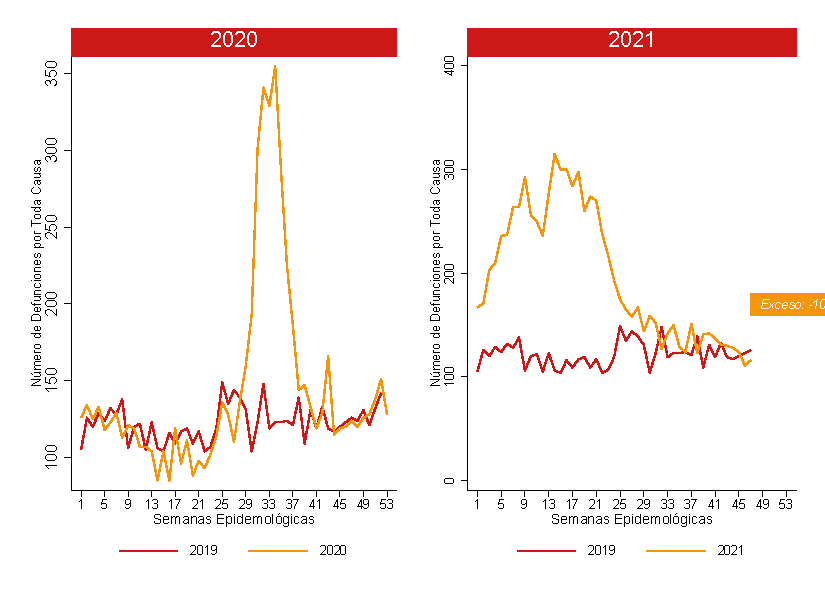
\includegraphics[width=0.85\linewidth]{../figuras/exceso_region.pdf}
	\end{center}
	{\footnotesize {Fuente de datos: SISCOVID, NOTICOVID.}}
	\end{figure}
\clearpage

	\subsection*{Cobertura de Vacunación por COVID-19 en la Región Cusco, hasta la SE 51.}
\noindent La Figura \ref{fig:vacuna_edad} muestra la cobertura de vacunación por grupo etario en la Región Cusco. El mayor porcentaje de cobertura se encuentra en el grupo etario de 70 a 79 años (con 86,5$\%$ de dos dosis de vacuna), seguido del grupo etario de 60 a 69 años  (con 85,4$\%$ con dos dosis de vacuna). La menor cobertura de vacunación se encuentra en el grupo etario de 20 a 29 años, con 52,3$\%$ de personas vacunadas con las dos dosis. 

\begin{figure}[h]
	\caption{Cobertura de Vacunación por Grupo Etario en la Región Cusco, hasta la SE 51. }\label{fig:vacuna_edad}
	\begin{center}
		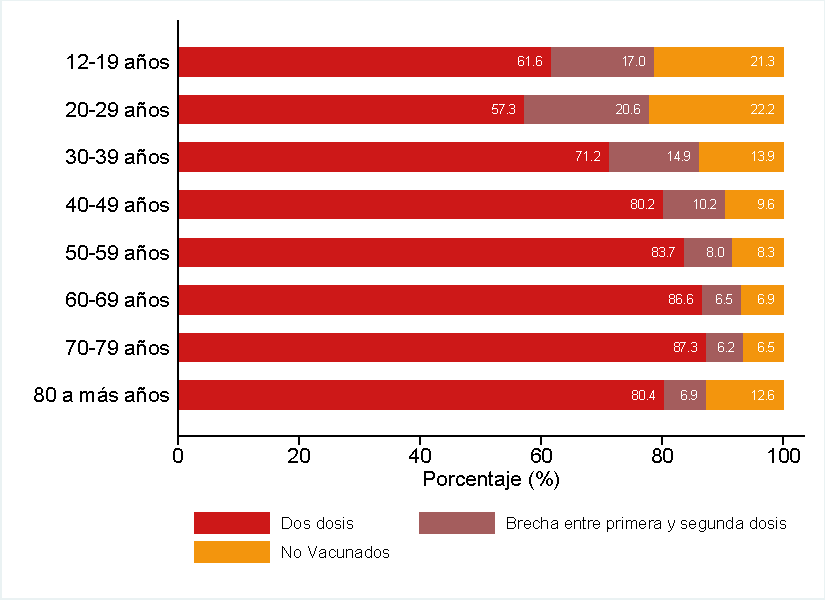
\includegraphics[width=0.65\linewidth]{../figuras/vacunacion_grupo_edad.pdf}
	\end{center}
	{\footnotesize {Fuente de datos: SICOVAC, HIS-MINSA.}}
\end{figure}

%La Figura \ref{fig:cobertura_vacunaci_provincia}  muestra la cobertura de vacunación en cada una de las provincias de Cusco por grupo etario. Es preciso señalar que la provincia de Espinar tiene la cobertura más baja de la región, en los grupos etarios desde los 50 años en adelante.
%
%\begin{figure}[h]
%	\caption{Cobertura de Vacunación por Provincia y por Grupo Etario en la Región Cusco, hasta la SE 51.}
%	\label{fig:cobertura_vacunaci_provincia}
%	\centering
%	\begin{subfigure}[b]{0.45\textwidth}
%		\centering
%		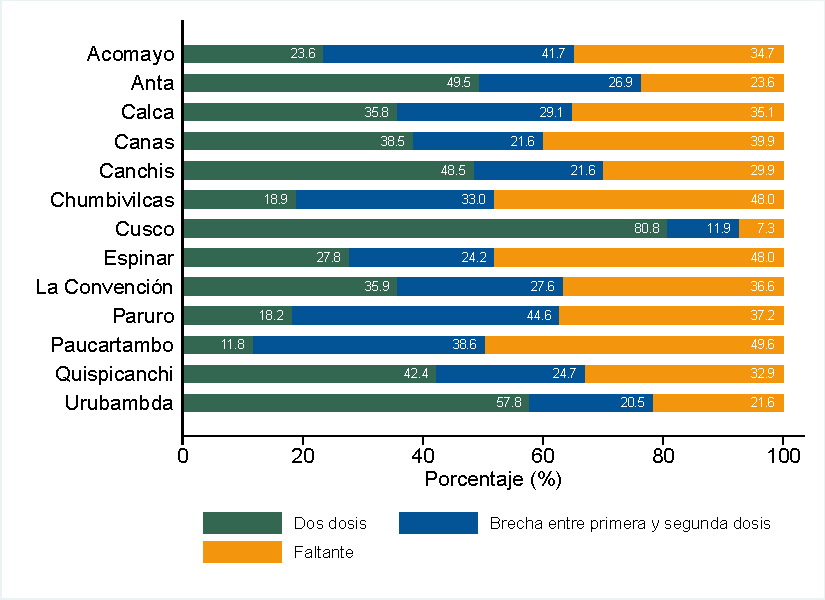
\includegraphics[width=\textwidth]{../figuras/vacunacion_provincial_edad_1}
%		\caption{ De 12 a 19 años}
%		%\label{fig:}
%	\end{subfigure}
%	\hfill
%	\begin{subfigure}[b]{0.45\textwidth}
%		\centering
%		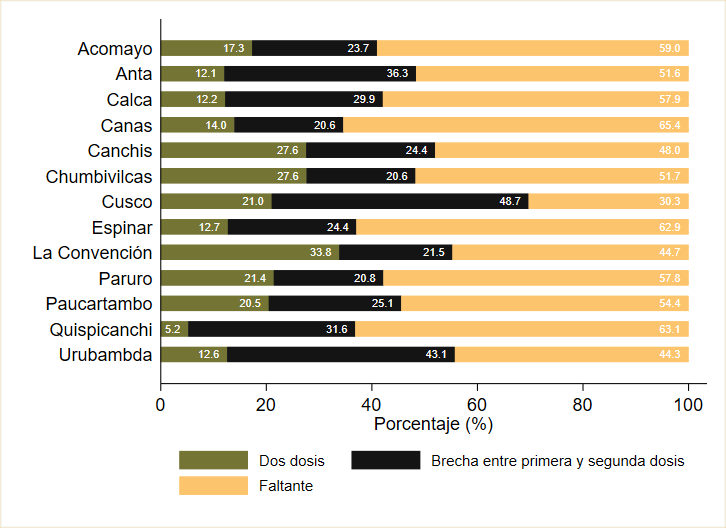
\includegraphics[width=\textwidth]{../figuras/vacunacion_provincial_edad_2}
%		\caption{De 20 a 29 años}
%		%\label{fig:70 a 79 años}
%	\end{subfigure}
%	\begin{subfigure}[b]{0.45\textwidth}
%		\centering
%		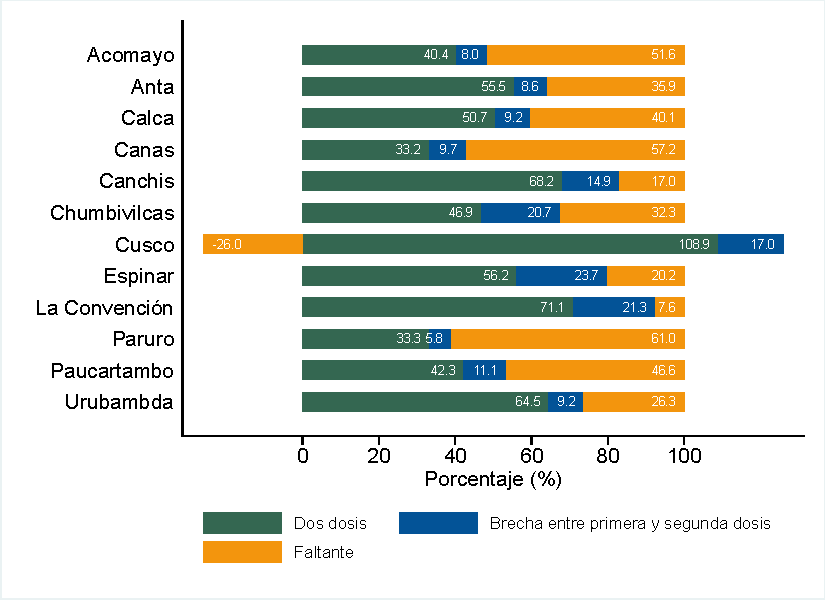
\includegraphics[width=\textwidth]{../figuras/vacunacion_provincial_edad_3}
%		\caption{De 30 a 39 años}
%		%\label{fig:60 a 69 años}
%	\end{subfigure}
%	\hfill
%	\begin{subfigure}[b]{0.45\textwidth}
%		\centering
%		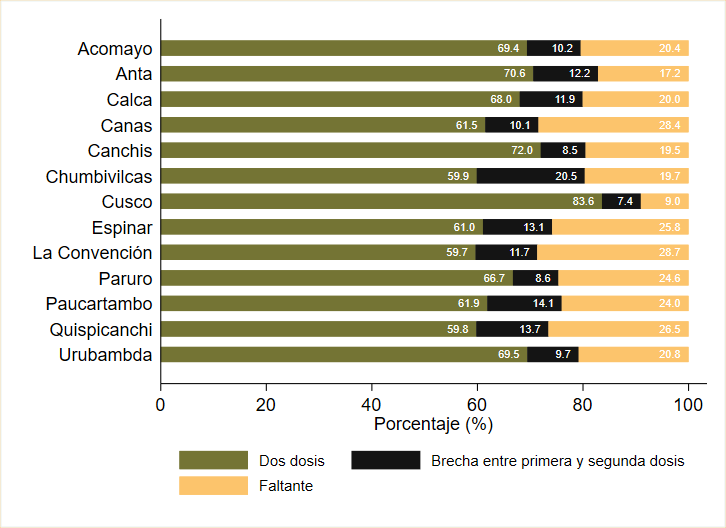
\includegraphics[width=\textwidth]{../figuras/vacunacion_provincial_edad_4}
%		\caption{De 40 a 49 años}
%		%\label{fig:50 a 59 años}
%	\end{subfigure}
%	\begin{subfigure}[b]{0.45\textwidth}
%		\centering
%		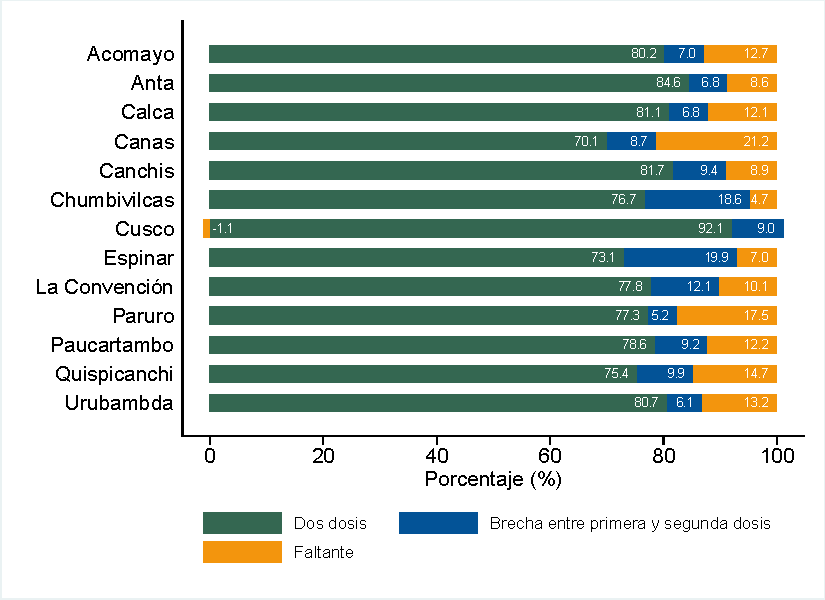
\includegraphics[width=\textwidth]{../figuras/vacunacion_provincial_edad_5}
%		\caption{De 50 a 59 años}
%		%\label{fig:40 a 49 años}
%	\end{subfigure}
%	\hfill
%	\begin{subfigure}[b]{0.45\textwidth}
%		\centering
%		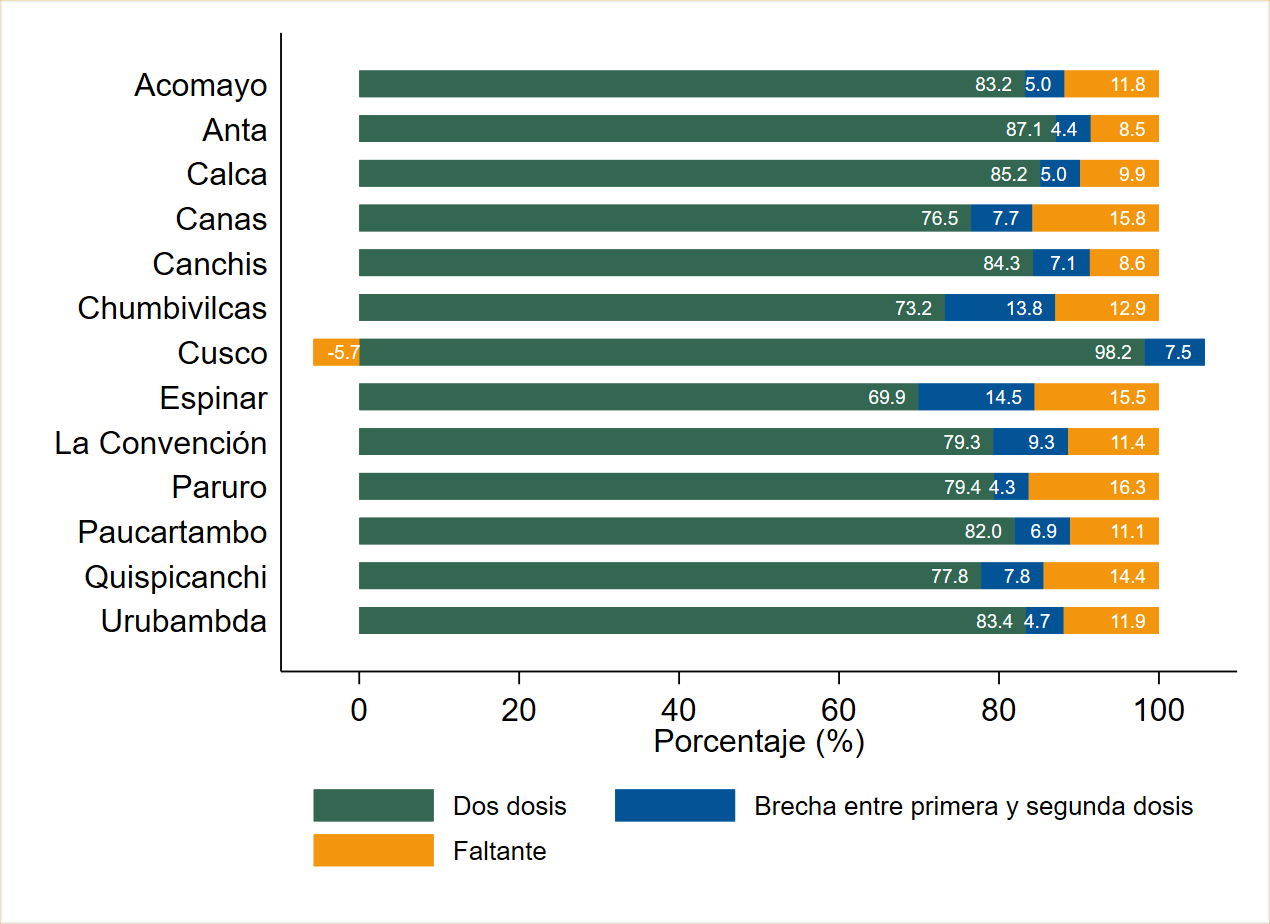
\includegraphics[width=\textwidth]{../figuras/vacunacion_provincial_edad_6}
%		\caption{De 60 a 69 años}
%		%\label{fig:40 a 49 años}
%	\end{subfigure}
%\begin{subfigure}[b]{0.45\textwidth}
%	\centering
%	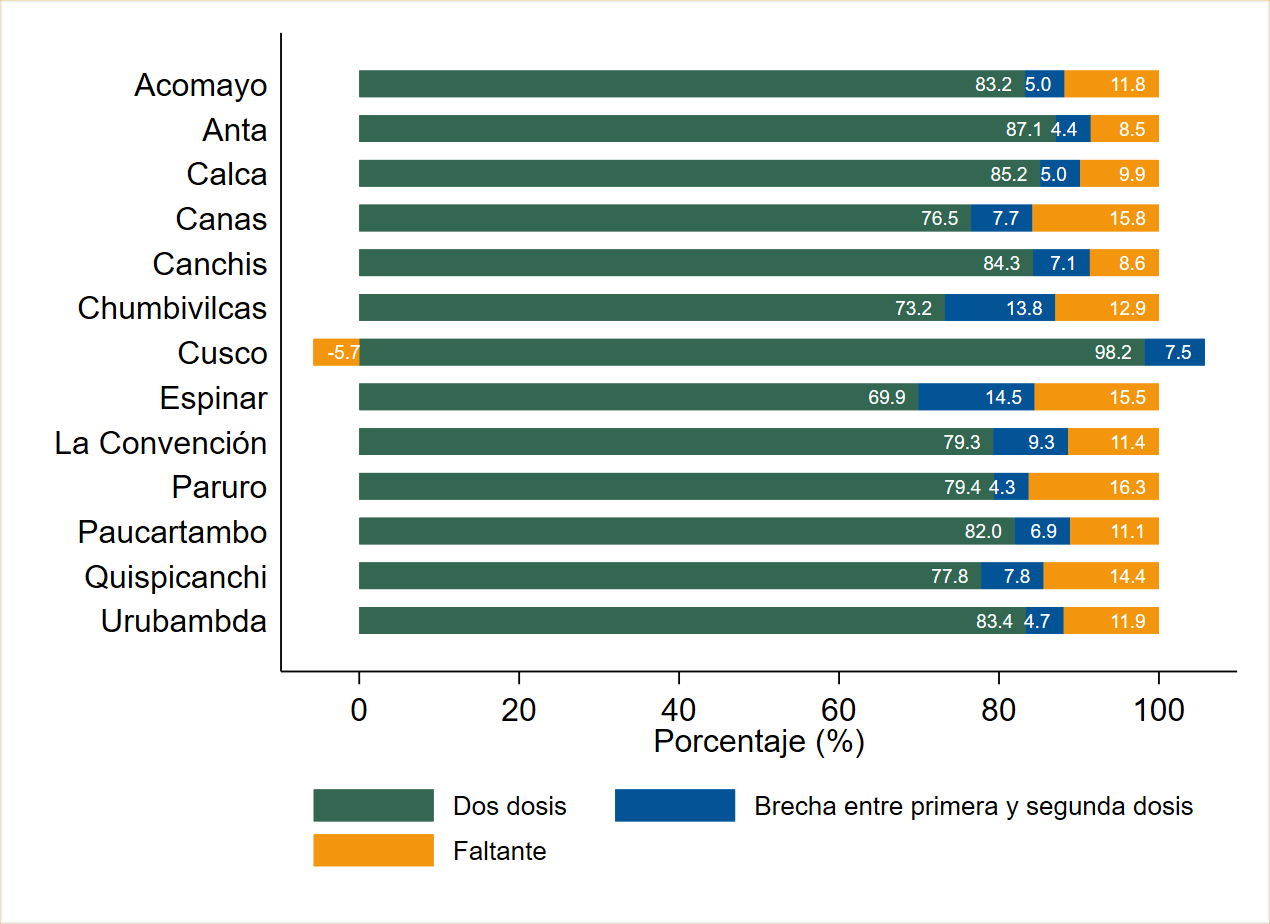
\includegraphics[width=\textwidth]{../figuras/vacunacion_provincial_edad_6}
%	\caption{De 70 a 79 años}
%	%\label{fig:40 a 49 años}
%\end{subfigure}
%\hfill
%\begin{subfigure}[b]{0.45\textwidth}
%	\centering
%	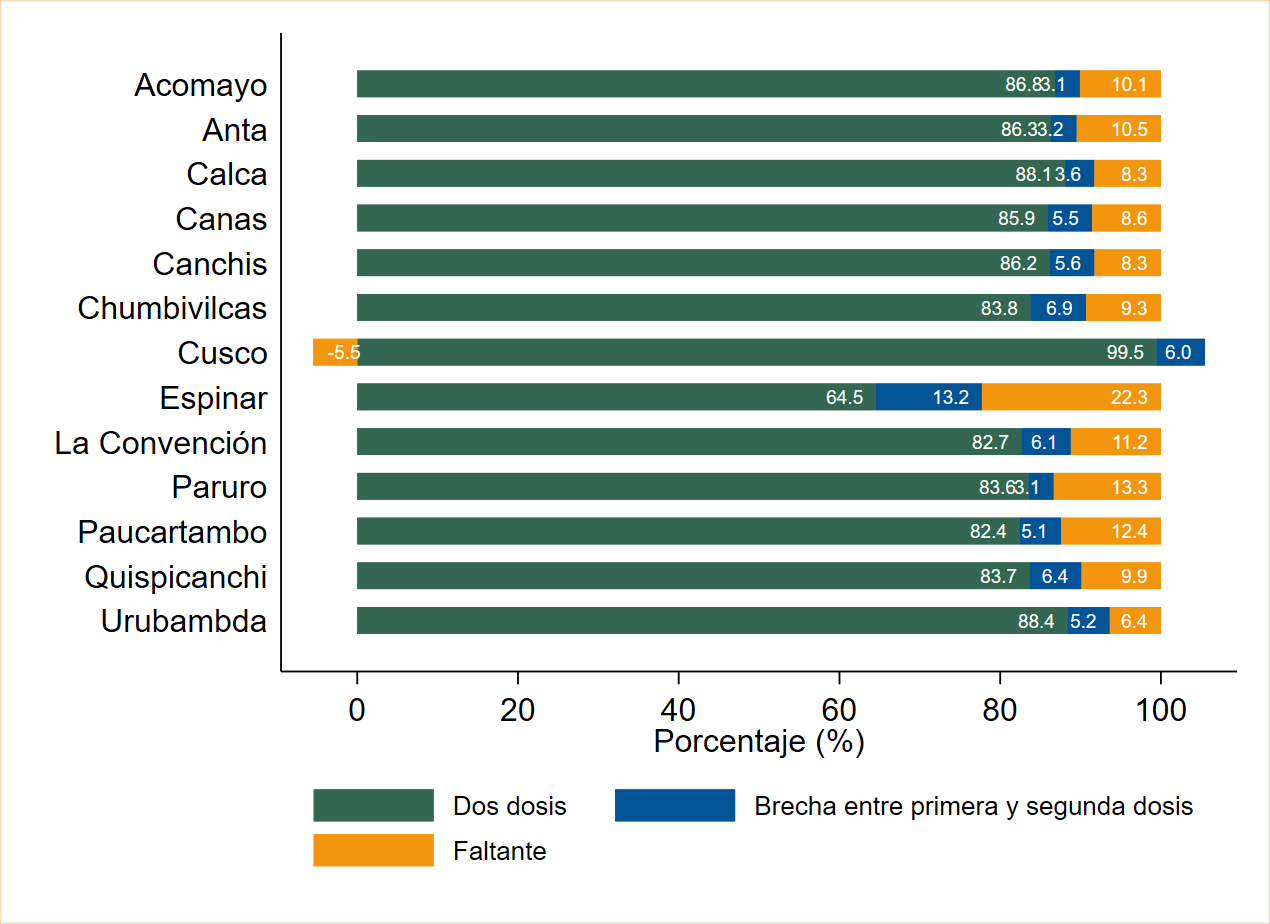
\includegraphics[width=\textwidth]{../figuras/vacunacion_provincial_edad_7}
%	\caption{Más de 80 años}
%	%\label{fig:40 a 49 años}
%\end{subfigure}
%\end{figure}

\clearpage
\subsection*{Ocupación de Camas}
\noindent La disponibilidad y ocupación de camas UCI se ve resumida en la Figura \ref{fig:ocupacion_uci}, se evidencia que para la SE 51 el número de camas UCI decreció a 28 (cuatro camas menos respecto a las semanas anteriores); sin embargo,  el porcentaje de ocupación descendió de 75$\%$ a 57$\%$ camas ocupadas.

\begin{figure}[h]
	\caption{Ocupación de Camas UCI COVID-19 en la Región Cusco, hasta la SE 51, 2021.}\label{fig:ocupacion_uci}
	\begin{center}
		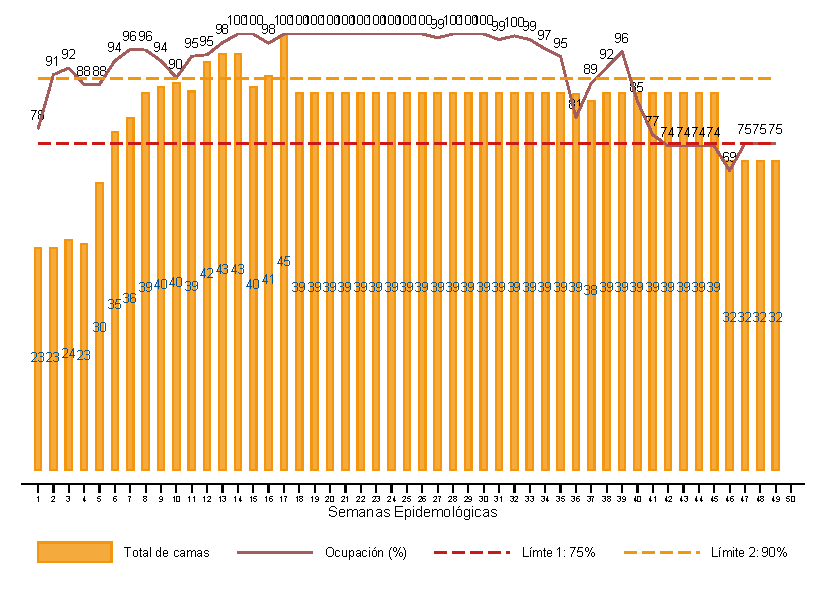
\includegraphics[width=0.95\linewidth]{../figuras/uci.pdf}
	\end{center}
	{\footnotesize {Fuente de datos: REFERENCIAS Y CONTRAREFERENCIAS.}}
\end{figure}
\cleardoublepage

En la Figura \ref{fig:ocupacion_3_nivel}, se plasma el porcentaje de ocupación y número de camas no-UCI COVID en el nivel Hospitalario III. Para la SE 51, el número de camas disponibles fue de 264, con un porcentaje bajo de ocupación de camas, quedando el 87$\%$ de camas disponibles para hospitalización. 
  
\begin{figure}[htpb]
	\caption{Ocupación de Camas no UCI COVID-19 en el nivel III en la Región Cusco, hasta la SE 51, 2021.}\label{fig:ocupacion_3_nivel}
	\begin{center}
		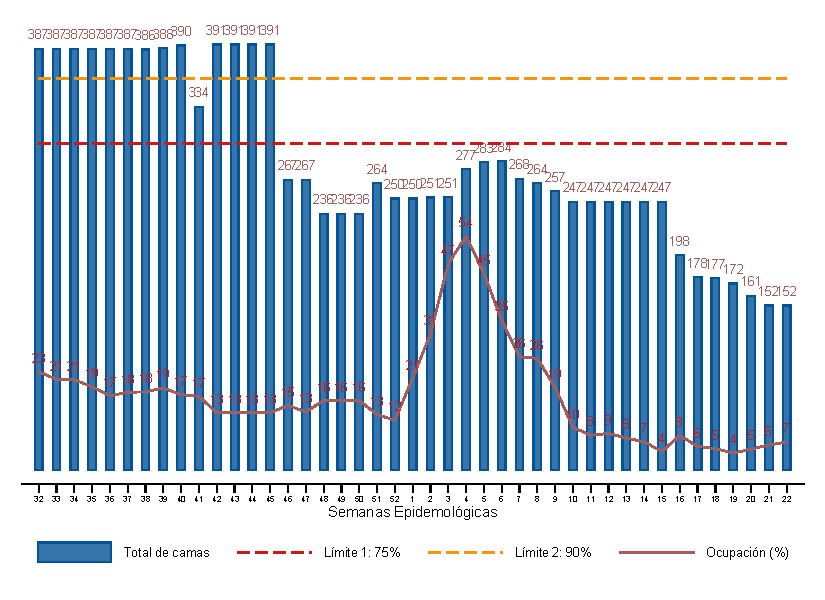
\includegraphics[width=0.95\linewidth]{../figuras/nivel_3.pdf}
	\end{center}
	{\footnotesize {Fuente de datos: REFERENCIAS Y CONTRAREFERENCIAS.}}
\end{figure}

\clearpage

En la Figura \ref{fig:ocupacion_2nivel}, se observa el número de camas disponibles y su porcentaje de ocupación en el Nivel II. Se evidencia que el porcentaje de ocupación de camas se mantiene bajo, siendo sólo del 8$\%$ para la SE 51. 

\begin{figure}[h]
	\caption{Disponibilidad y Ocupación de Camas-COVID a Nivel de Hospitales del Nivel II en la Región Cusco, hasta la SE 51, 2021}\label{fig:ocupacion_2nivel}
	\begin{center}
		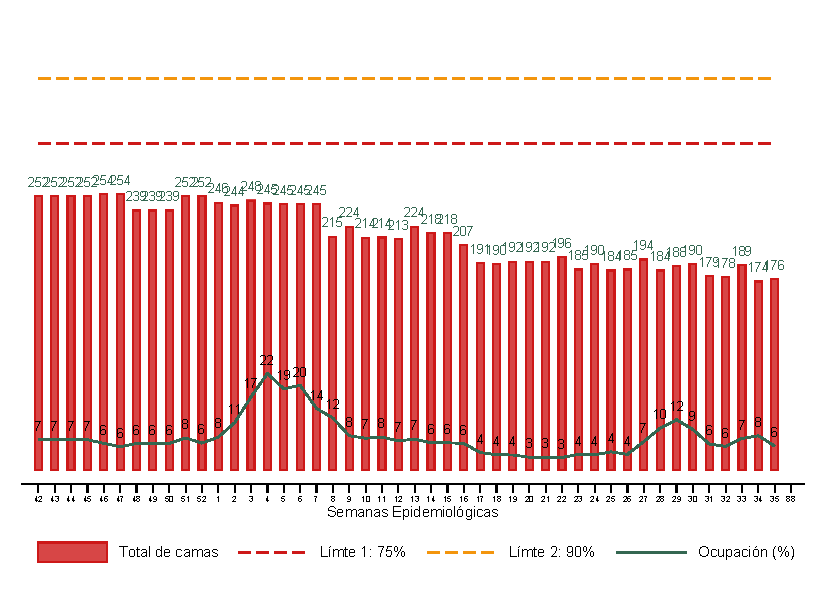
\includegraphics[width=0.95\linewidth]{../figuras/nivel_2.pdf}
	\end{center}
	{\footnotesize {Fuente de datos: REFERENCIAS Y CONTRAREFERENCIAS.}}
\end{figure}
\clearpage
\begin{landscape}
	
	\subsection*{Evaluación Provincial de la Infección por COVID-19} 
	
	\begin{tabular}{@{}lrrrrr@{}}
	\rowcolor[HTML]{ECF4FF} 
	\textbf{Provincias}                   & \multicolumn{1}{l}{\cellcolor[HTML]{ECF4FF}\textbf{población}} & \multicolumn{1}{l}{\cellcolor[HTML]{ECF4FF}\textbf{Pruebas Totales}} & \multicolumn{1}{l}{\cellcolor[HTML]{ECF4FF}\textbf{Funciones}} & \multicolumn{1}{l}{\cellcolor[HTML]{ECF4FF}\textbf{Tasa de letalidad}} & \multicolumn{1}{l}{\cellcolor[HTML]{ECF4FF}\textbf{\begin{tabular}[c]{@{}l@{}}tasa de mortalidad x \\   100.000 hab\end{tabular}}} \\
	\cellcolor[HTML]{FD6864}CANCHIS       & 105,049                                                        & 1,545                                                                & 5                                                              & 0.3\%                                                                  & 4.8                                                                                                                                \\
	\cellcolor[HTML]{FD6864}PAUCARTAMBO   & 52,989                                                         & 301                                                                  & 2                                                              & 0.7\%                                                                  & 3.8                                                                                                                                \\
	\cellcolor[HTML]{FD6864}LA CONVENCION & 185,793                                                        & 2,623                                                                & 7                                                              & 0.3\%                                                                  & 3.8                                                                                                                                \\
	\cellcolor[HTML]{FFFC9E}CUSCO         & 463,656                                                        & 16,911                                                               & 9                                                              & 0.1\%                                                                  & 1.9                                                                                                                                \\
	\cellcolor[HTML]{FFFC9E}ESPINAR       & 71,304                                                         & 479                                                                  & 1                                                              & 0.2\%                                                                  & 1.4                                                                                                                                \\
	\cellcolor[HTML]{FFFC9E}CALCA         & 76,462                                                         & 462                                                                  & 1                                                              & 0.2\%                                                                  & 1.3                                                                                                                                \\
	\cellcolor[HTML]{9AFF99}CHUMBIVILCAS  & 84,925                                                         & 448                                                                  & 1                                                              & 0.2\%                                                                  & 1.2                                                                                                                                \\
	\cellcolor[HTML]{9AFF99}QUISPICANCHI  & 92,566                                                         & 735                                                                  & 1                                                              & 0.1\%                                                                  & 1.1                                                                                                                                \\
	\cellcolor[HTML]{9AFF99}ACOMAYO       & 28,477                                                         & 149                                                                  & 0                                                              & 0.0\%                                                                  & 0.0                                                                                                                                \\
	\cellcolor[HTML]{9AFF99}ANTA          & 57,731                                                         & 480                                                                  & 0                                                              & 0.0\%                                                                  & 0.0                                                                                                                                \\
	\cellcolor[HTML]{9AFF99}CANÁS         & 40,420                                                         & 206                                                                  & 0                                                              & 0.0\%                                                                  & 0.0                                                                                                                                \\
	\cellcolor[HTML]{9AFF99}PARURO        & 31,264                                                         & 132                                                                  & 0                                                              & 0.0\%                                                                  & 0.0                                                                                                                                \\
	\cellcolor[HTML]{9AFF99}URUBAMBÁ      & 66,439                                                         & 900                                                                  & 0                                                              & 0.0\%                                                                  & 0.0                                                                                                                                \\
	& \multicolumn{1}{l}{}                                           & \multicolumn{1}{l}{}                                                 & \multicolumn{1}{l}{}                                           & \multicolumn{1}{l}{}                                                   & \multicolumn{1}{l}{}                                                                                                               \\
	\rowcolor[HTML]{ECF4FF} 
	\textbf{Totales generales}            & \textbf{1,357,075}                                             & \textbf{25,371}                                                      & \textbf{27}                                                    & \textbf{0.11\%}                                                        & \textbf{2.0}                                                                                                                      
\end{tabular}
	{\footnotesize Fuente de datos: NOTICOVID, SISCOVID, SINADEF.}
	
	\noindent El Cuadro muestra la tasa de letalidad y mortalidad de todas las provincias de la Región Cusco. Se presentan las provincias ordenadas de mayor a menor tasa de mortalidad, encontrándose la mayor tasa (279.9 defunciones/ 100 000 habitantes) en Canchis. 
	
\end{landscape}
%---------------------------------------------------------------------------
% CAPÍTULO: EVALUACIÓN DE PROVINCIAS
%---------------------------------------------------------------------------

%insertar el cover del capitulo
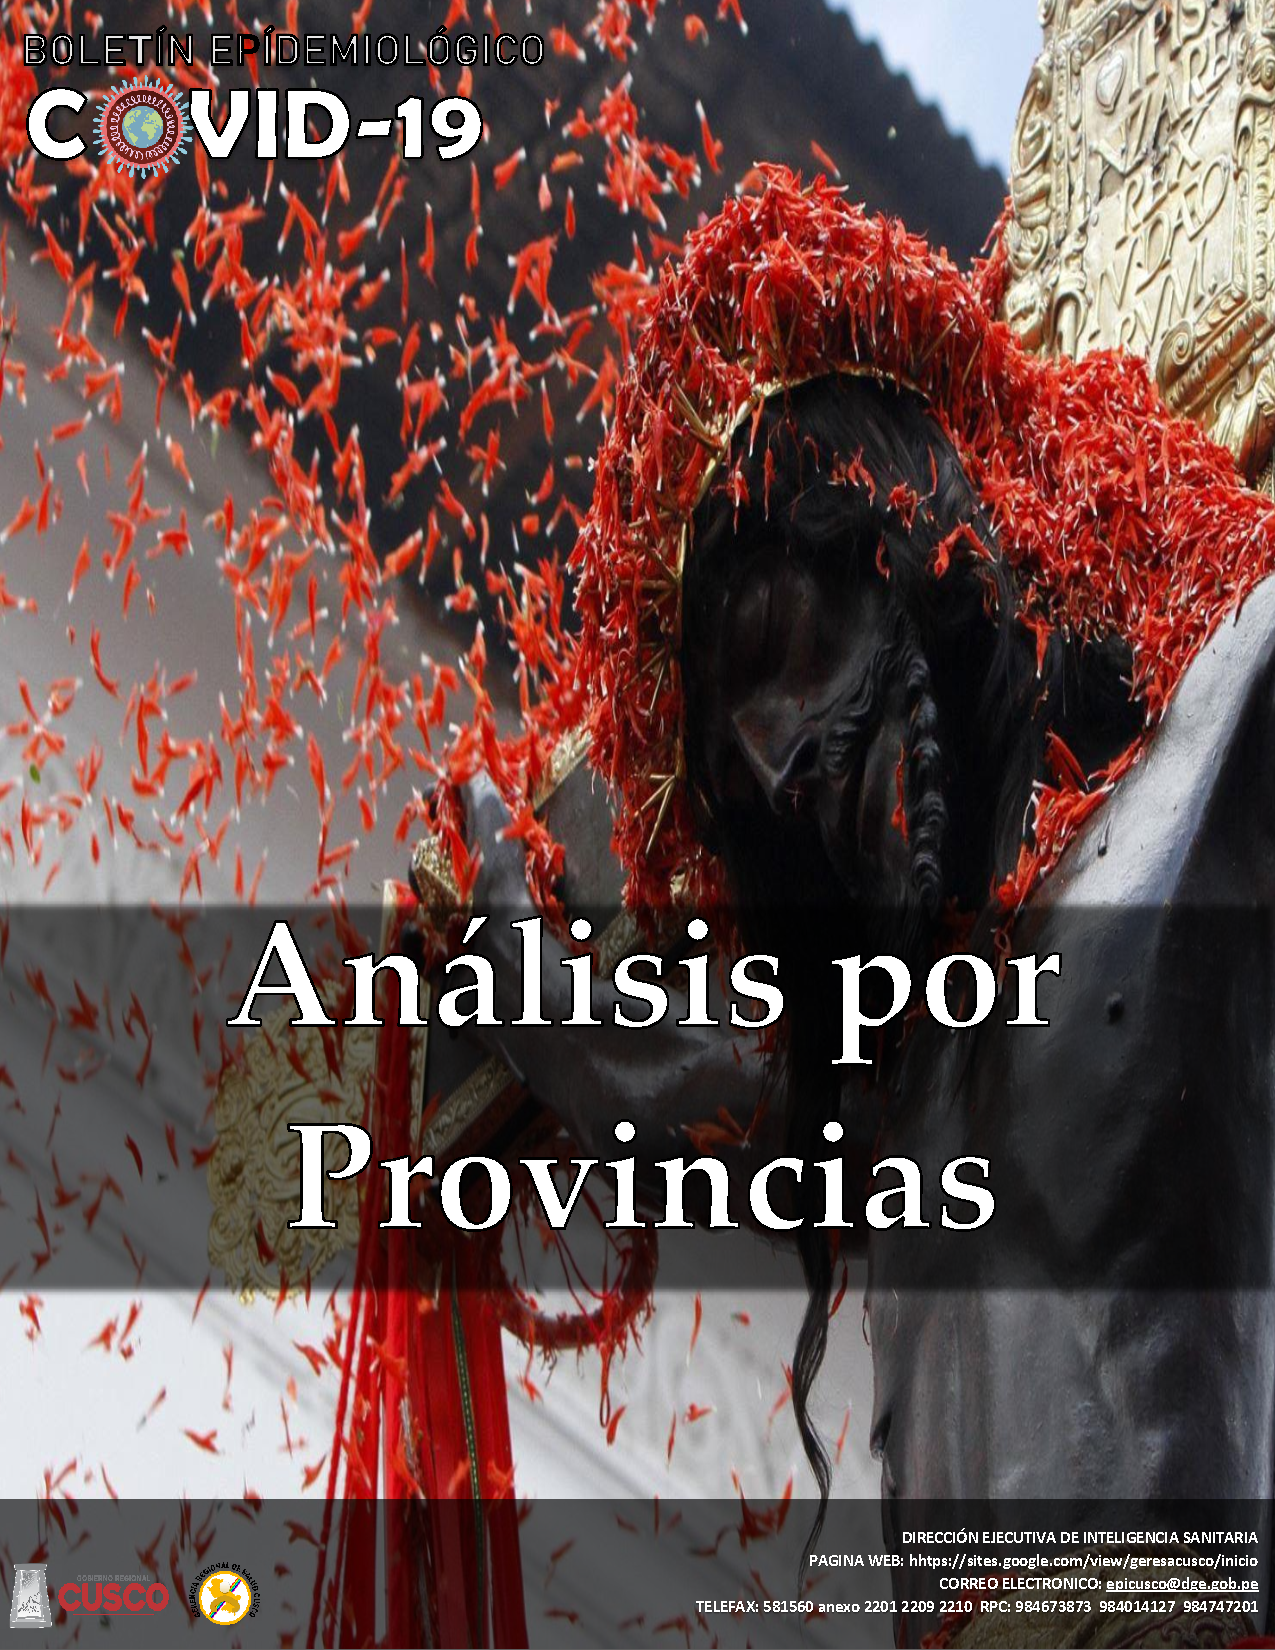
\includepdf[pages={1}]{../editorial/5.pdf}
\clearpage

	\section*{Evaluación para Provincias Priorizadas}
\addcontentsline{toc}{chapter}{Evaluación para Provincias Priorizadas}
\noindent La Figura \ref{fig:incidencia_provincias} muestra las tasas de incidencia acumulada por provincia, ordenadas de mayor a menor. Se observa que la provincia de Cusco tiene la tasa de incidencia acumulada más alta (580,6 casos /10 000* personas), seguida de la provincia de La Convención (327,4 casos/10 000*personas).

\begin{figure}[!htpb]
	\caption{Tasa de Incidencia Acumulada por Provincia en la Región Cusco, hasta el 26 de diciembre del 2021 *. }\label{fig:incidencia_provincias}
	\begin{center}
		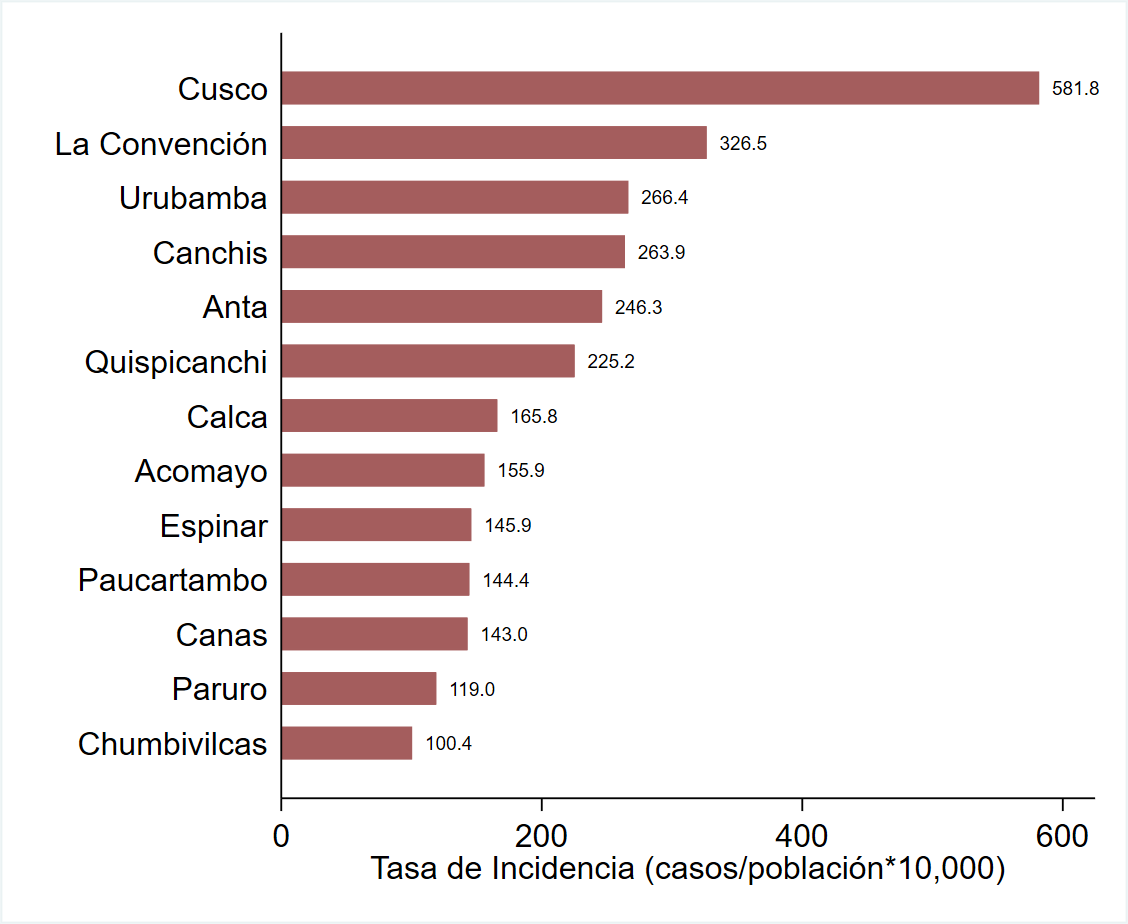
\includegraphics[width=0.75\linewidth]{../figuras/incidencia_provincial}
	\end{center}
	{\footnotesize {(*)Se consideró como caso positivo sólo a pacientes con prueba molecular o prueba antigénica positiva. 
			
	Fuente de datos: SISCOVID, NOTICOVID.}}
\end{figure}


La Figura \ref{fig:mortalidad_ordenada} muestra a las provincias de la región ordenadas de mayor a menor según la tasa de mortalidad acumulada. Se evidencia que la provincia de Canchis aún es la provincia con mayor tasa de mortalidad acumulada con 28,1 defunciones / 10 000* personas.  

\begin{figure}[h]
	\caption{Tasa de Mortalidad Acumulada por Provincia en la Región Cusco, hasta el 25 de diciembre del 2021. }\label{fig:mortalidad_ordenada}
	\begin{center}
		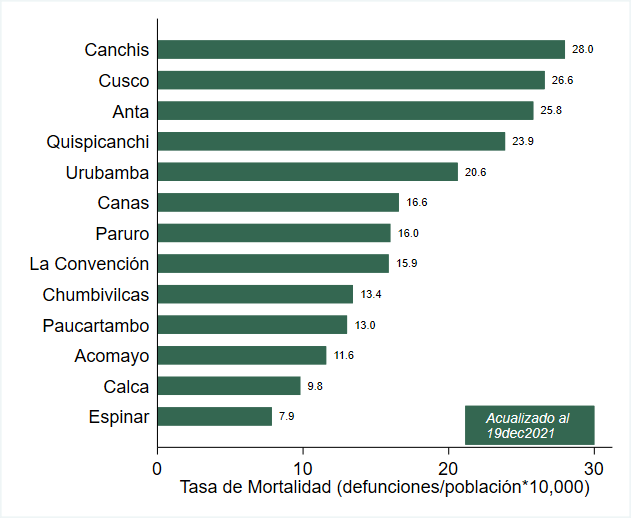
\includegraphics[width=0.65\linewidth]{../figuras/mortalidad_provincial}
	\end{center}
	{\footnotesize {Fuente de datos: SISCOVID, NOTICOVID.}}
\end{figure}

La Figura \ref{fig:incidencia_provincial} muestra la tendencia de la incidencia acumulada a través del año. En las últimas dos semanas, la pendiente se crecimiento se ha mantenido en meceta. 
%
\begin{figure}[h]
	\caption{Tendencia Provincial de Incidencia acumulada de COVID-19, hasta la SE 51, 2021. }\label{fig:incidencia_provincial}
	\begin{center}
		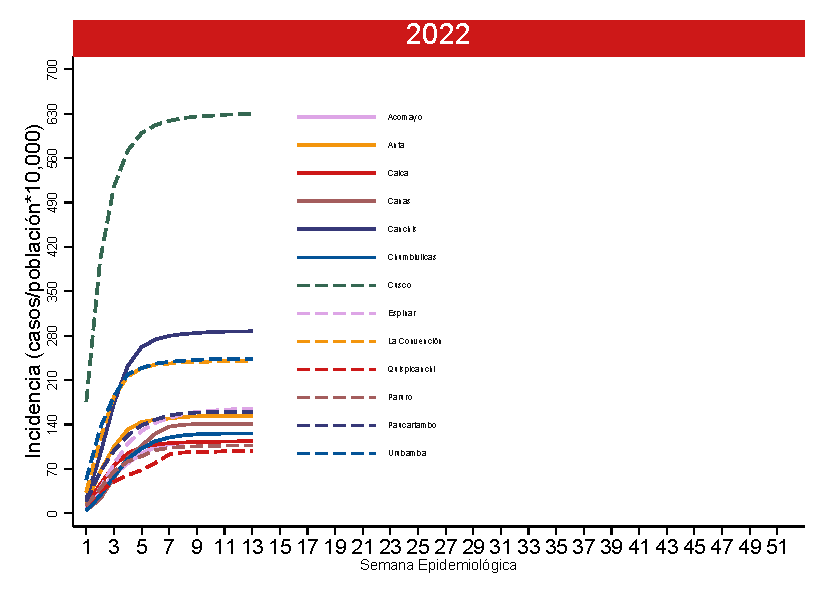
\includegraphics[width=0.65\linewidth]{../figuras/incidencia_provincial_2021.pdf}
	\end{center}
	{\footnotesize {Fuente de datos: SINADEF.}}
\end{figure}

\clearpage
	
\section*{Evaluación Provincial de 5 Indicadores}
		\noindent El objetivo de estas figuras es comparar a cada provincia consigo misma de acuerdo a su historia  en la primera ola (en el año 2020). Se evaluaron los siguientes indicadores: incidencia (tomando en cuenta pruebas moleculares y antigénicas), tasa de mortalidad, tasa de positividad por prueba molecular, tasa de positividad por prueba antigénica, y exceso de defunciones para cada provincia.
		
		\subsection*{Provincia de Acomayo}
		\noindent La figura (Figura \ref{fig:inc_mort_acomayo}),  muestra un descenso de la tasa de mortalidad e incidencia a partir de la SE 37, el cual se ha mantenido hasta la fecha. 
		\noindent La figura (Figura\ref{fig:positividad_acomayo}) muestra un descenso de la tasa de positividad de pruebas moleculares y antigénicas desde la SE 37.
		
		 En la Figura \ref{fig:exceso_acomayo} se muestra que hay un exceso de menos 1 defunción (exceso negativo) respecto al año 2019.
		
		\begin{figure}[h]
			\caption{Tasa de Incidencia y Mortalidad Comparativa en la Provincia de Acomayo 2020 y 2021, hasta la SE 51.}\label{fig:inc_mort_acomayo}
			\begin{center}
				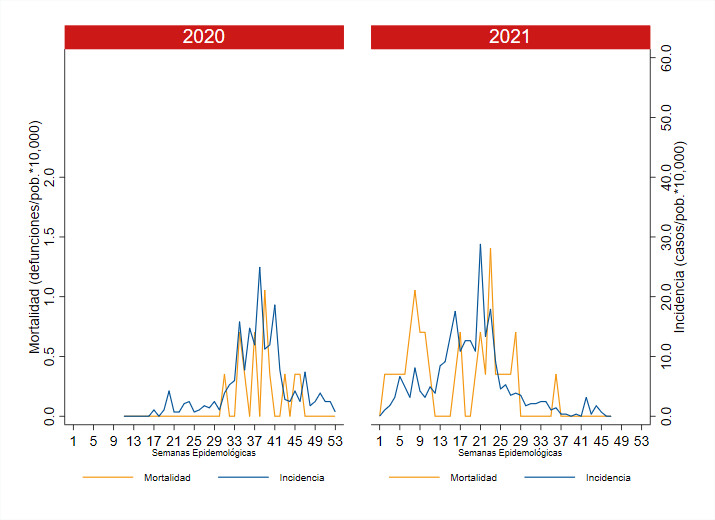
\includegraphics[width=0.65\linewidth]{../figuras/incidencia_mortalidad_20_21_1}
			\end{center}
			{\footnotesize {Fuente de datos: NOTICOVID, SISCOVID, SINADEF.}}
		\end{figure}
		
		\begin{figure}[h]
			\caption{Tasa de Positividad de Prueba Molecular y Antigénica Comparativa en la Provincia de Acomayo 2020 y 2021, hasta la SE 51. }\label{fig:positividad_acomayo}
			\begin{center}
				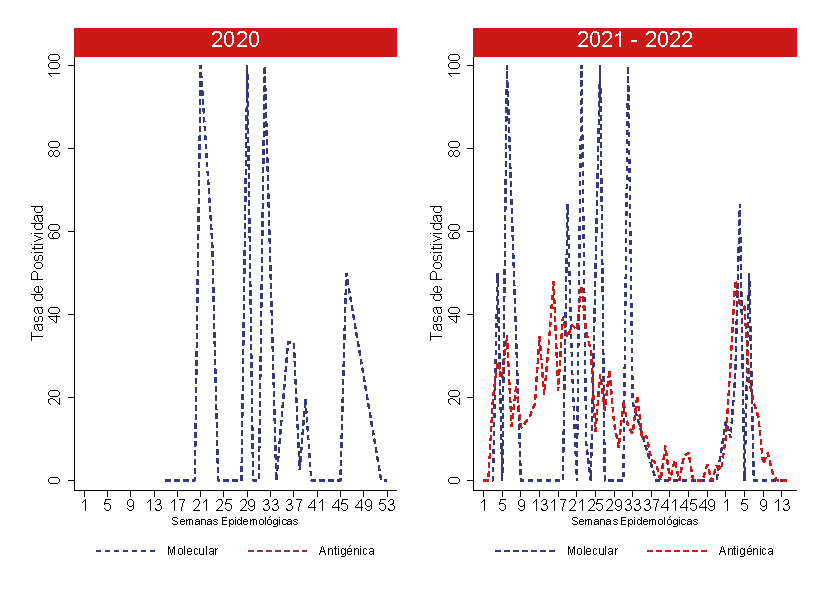
\includegraphics[width=0.7\linewidth]{../figuras/positividad_20_21_1}
			\end{center}
			{\footnotesize {Fuente de datos: NOTICOVID, SISCOVID.}}
		\end{figure}
		
		\begin{figure}[h]
			\caption{Exceso de Defunciones Comparativo en la Provincia de Acomayo 2020 y 2021, hasta la SE 51.}\label{fig:exceso_acomayo}
			\begin{center}
				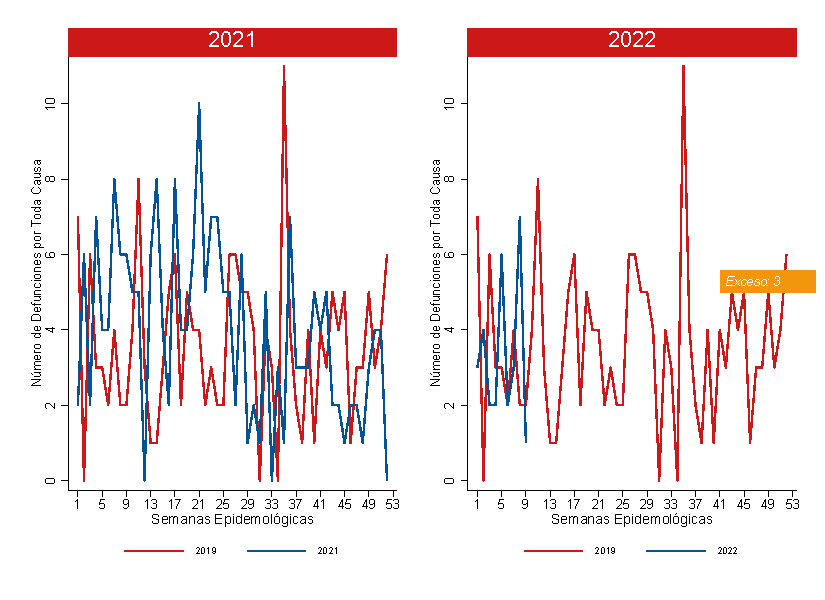
\includegraphics[width=0.7\linewidth]{../figuras/exceso_1}
			\end{center}
			{\footnotesize {Fuente de datos: SINADEF.}}
		\end{figure}
		
		% Anta
		\clearpage
		
		\subsection*{Provincia de Anta}
		\noindent La figura (Figura \ref{fig:inc_mort_anta}),  muestra un descenso de la tasa de mortalidad e incidencia a partir de la SE 26, el cual se ha mantenido hasta la fecha. 
		\noindent La figura (Figura\ref{fig:positividad_anta}) muestra una tendencia variable de la tasa de positividad de pruebas moleculares y antigénicas.
		
		En la Figura \ref{fig:exceso_anta} se muestra que hay un exceso de defunciones de 6 (exceso positivo) respecto al año 2019.
		
		\begin{figure}[h]
			\caption{Tasa de Incidencia y Mortalidad Comparativa en la Provincia de Anta 2020 y 2021, hasta la SE 51.}\label{fig:inc_mort_anta}
			\begin{center}
				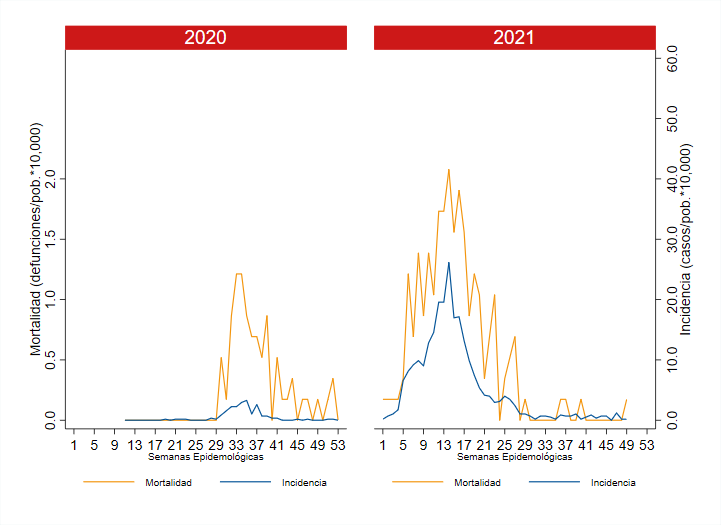
\includegraphics[width=0.7\linewidth]{../figuras/incidencia_mortalidad_20_21_2}
			\end{center}
			{\footnotesize {Fuente de datos: NOTICOVID, SISCOVID, SINADEF.}}
		\end{figure}
		
		\begin{figure}[h]
			\caption{Tasa de Positividad de Prueba Molecular y Antigénica Comparativa en la Provincia de Anta 2020 y 2021, hasta la SE 51.}\label{fig:positividad_anta}
			\begin{center}
				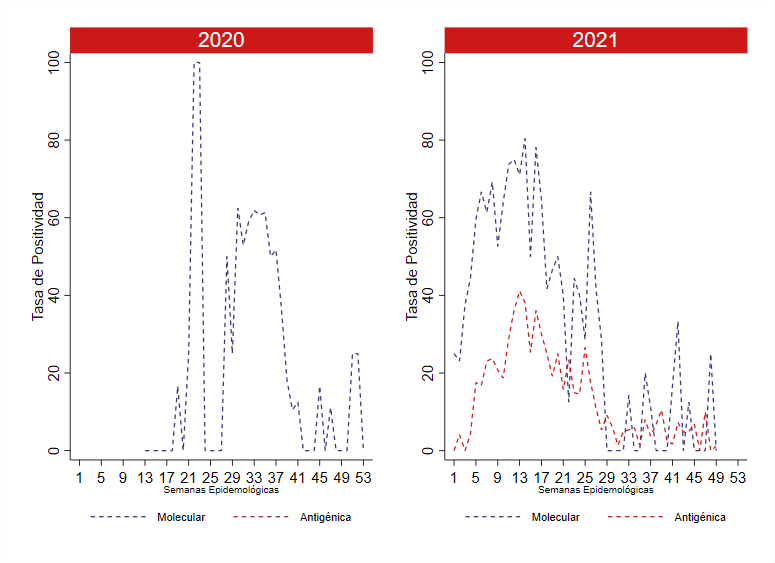
\includegraphics[width=0.7\linewidth]{../figuras/positividad_20_21_2}
			\end{center}
			{\footnotesize {Fuente de datos: NOTICOVID, SISCOVID.}}
		\end{figure}
		
		\begin{figure}[h]
			\caption{Exceso de Defunciones Comparativo en la Provincia de Anta  2020 y 2021, hasta la SE 51.}\label{fig:exceso_anta}
			\begin{center}
				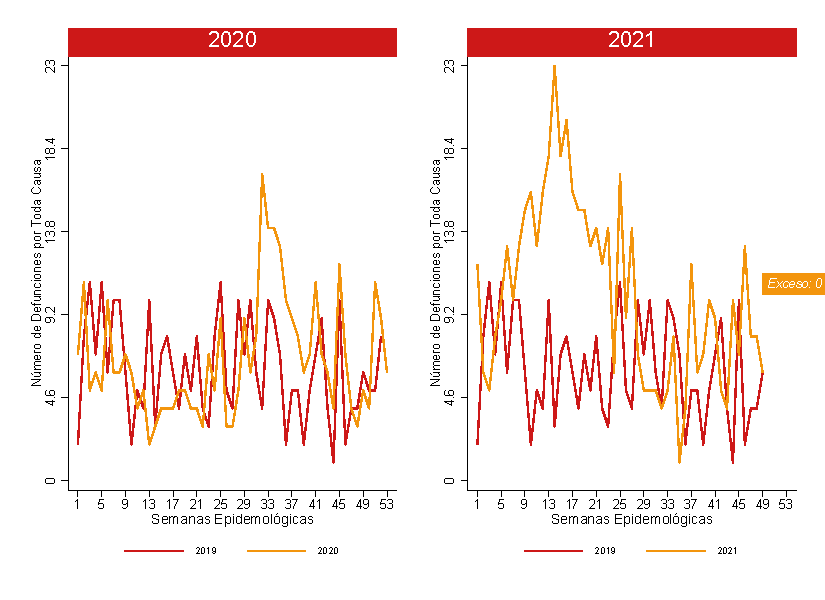
\includegraphics[width=0.7\linewidth]{../figuras/exceso_2}
			\end{center}
			{\footnotesize {Fuente de datos: SINADEF.}}
		\end{figure}
		
		% Canas
		\clearpage
		
		\subsection*{Provincia de Canas}
		\noindent La figura (Figura \ref{fig:inc_mort_canas}),  muestra un descenso de la tasa de mortalidad e incidencia a partir de la SE 26, el cual se ha mantenido hasta la fecha. 
		\noindent La figura (Figura\ref{fig:positividad_canas}) muestra una tendencia variable de la tasa de positividad de pruebas moleculares y antigénicas.
		
		La Figura \ref{fig:exceso_canas} muestra que hay un exceso de menos 3 defunciones ( exceso negativo) respecto al año 2019.
		
		\begin{figure}[h]
			\caption{Tasa de Incidencia y Mortalidad Comparativa en la Provincia de Canas 2020 y 2021, hasta la SE 51.}\label{fig:inc_mort_canas}
			\begin{center}
				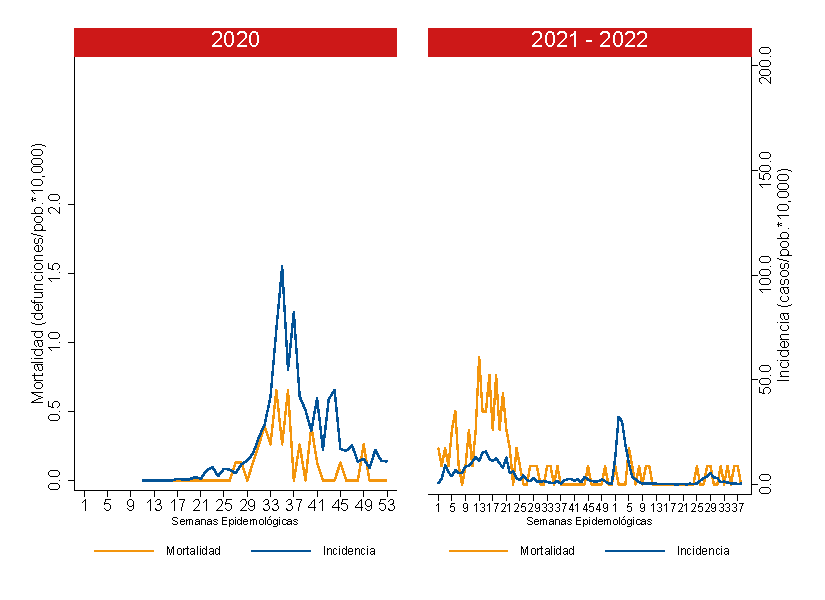
\includegraphics[width=0.7\linewidth]{../figuras/incidencia_mortalidad_20_21_3}
			\end{center}
			{\footnotesize {Fuente de datos: NOTICOVID, SISCOVID, SINADEF.}}
		\end{figure}
		
		\begin{figure}[h]
			\caption{Tasa de Positividad de Prueba Molecular y Antigénica Comparativa en la Provincia de Canas 2020 y 2021, hasta la SE 51.}\label{fig:positividad_canas}
			\begin{center}
				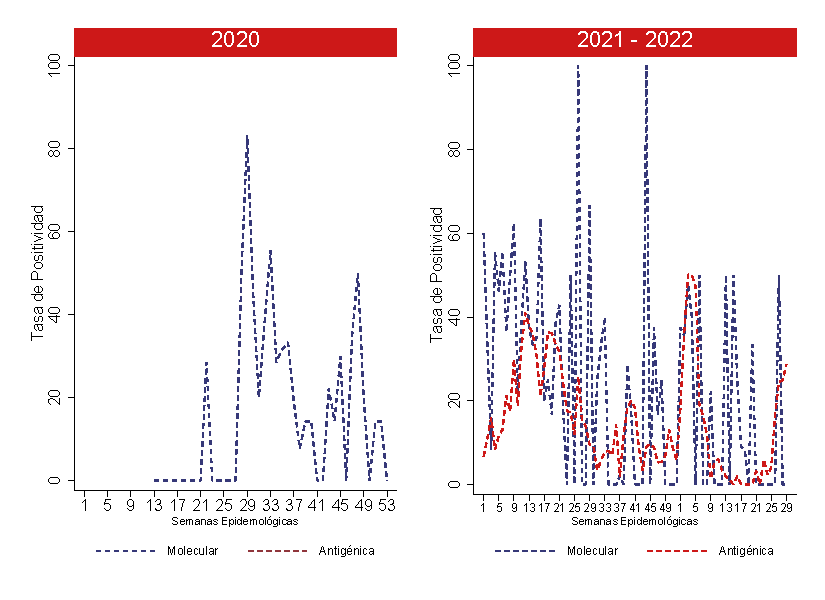
\includegraphics[width=0.7\linewidth]{../figuras/positividad_20_21_3}
			\end{center}
			{\footnotesize {Fuente de datos: NOTICOVID, SISCOVID.}}
		\end{figure}
		
		\begin{figure}[h]
			\caption{Exceso de Defunciones Comparativo en la Provincia de Canas 2020 y 2021, hasta la SE 51.}\label{fig:exceso_canas}
			\begin{center}
				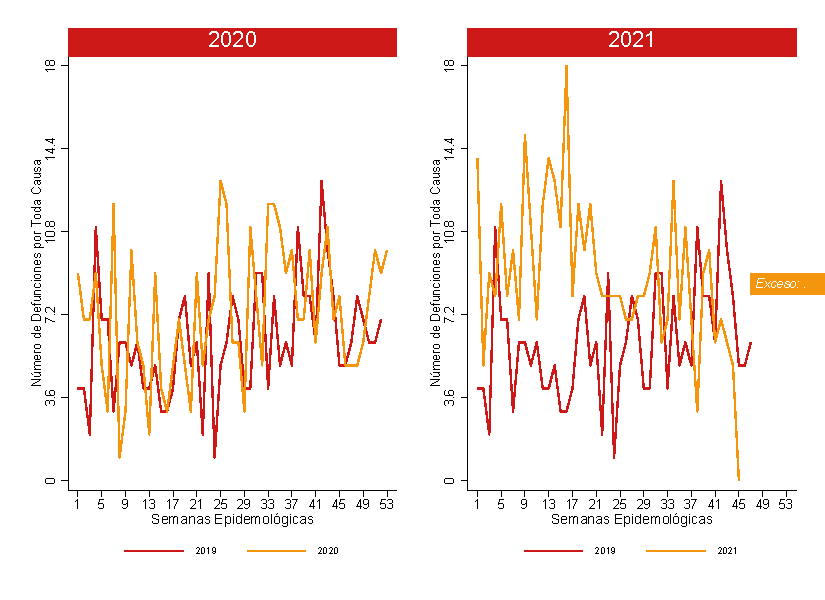
\includegraphics[width=0.7\linewidth]{../figuras/exceso_3}
			\end{center}
			{\footnotesize {Fuente de datos: SINADEF.}}
		\end{figure}
		
		% Calca
		\clearpage
		
		\subsection*{Provincia de Calca}
		\noindent Las figuras de abajo (Figura \ref{fig:inc_mort_calca}, \ref{fig:positividad_calca}) muestran el comportamiento de la tasa de incidencia, mortalidad y  positividad. Con respecto a la tasa de incidencia, se evidencia una tendencia al descenso desde la SE 29, con incremento discreto de casos entre semanas. En relación a la tasa de mortalidad, se reportaron muertes durante la SE 48.
		
		En la Figura \ref{fig:exceso_calca} se muestra que hay un exceso de menos una defunción (exceso negativo) respecto al año 2019.
		
		\begin{figure}[h]
			\caption{Tasa de Incidencia y Mortalidad Comparativa en la Provincia de Calca 2020 y 2021, hasta la SE 51.}\label{fig:inc_mort_calca}
			\begin{center}
				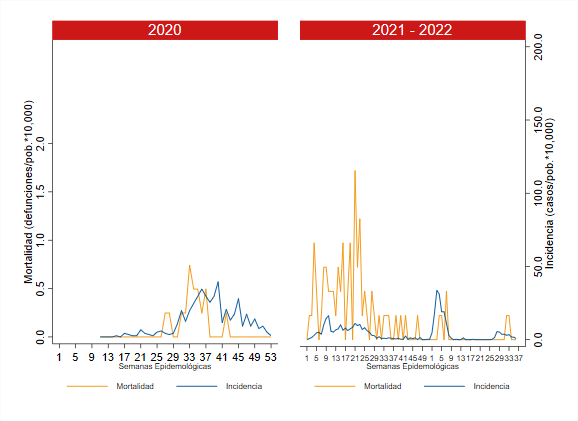
\includegraphics[width=0.7\linewidth]{../figuras/incidencia_mortalidad_20_21_4}
			\end{center}
			{\footnotesize {Fuente de datos: NOTICOVID, SISCOVID, SINADEF.}}
		\end{figure}
		
		\begin{figure}[h]
			\caption{Tasa de Positividad de Prueba Molecular y Antigénica Comparativa en la Provincia de Calca 2020 y 2021, hasta la SE 51.}\label{fig:positividad_calca}
			\begin{center}
				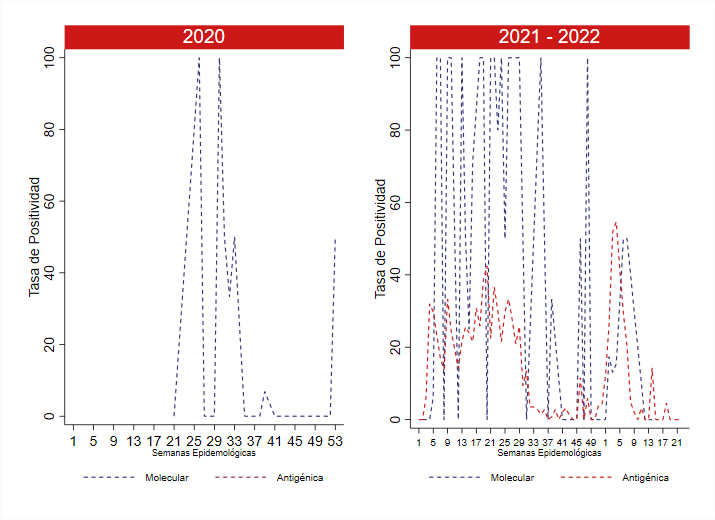
\includegraphics[width=0.7\linewidth]{../figuras/positividad_20_21_4}
			\end{center}
			{\footnotesize {Fuente de datos: NOTICOVID, SISCOVID.}}
		\end{figure}
		
		\begin{figure}[h]
			\caption{Exceso de Defunciones Comparativo en la Provincia de Calca 2020 y 2021, hasta la SE 51.}\label{fig:exceso_calca}
			\begin{center}
				\includegraphics[width=0.7\linewidth]{../figuras/exceso_4}
			\end{center}
			{\footnotesize {Fuente de datos: SINADEF.}}
		\end{figure}
		
		% Canas
		\clearpage
		
		\subsection*{Provincia de Canchis}
		\noindent La figura (Figura \ref{fig:inc_mort_canchis}),  muestra un descenso de la tasa de mortalidad e incidencia a partir de la SE 26, el cual se ha mantenido hasta la fecha. 
		\noindent La figura (Figura\ref{fig:positividad_canchis}) muestra una tendencia variable de la tasa de positividad de pruebas moleculares y antigénicas.
		
		En la Figura \ref{fig:exceso_canchis} se muestra que hay exceso de menos 7 defunciones (exceso negativo) respecto al año 2019.
		
		\begin{figure}[h]
			\caption{Tasa de Incidencia y Mortalidad Comparativa en la Provincia de Canchis 2020 y 2021, hasta la SE 51.}\label{fig:inc_mort_canchis}
			\begin{center}
				\includegraphics[width=0.7\linewidth]{../figuras/incidencia_mortalidad_20_21_5}
			\end{center}
			{\footnotesize {Fuente de datos: NOTICOVID, SISCOVID, SINADEF.}}
		\end{figure}
		
		\begin{figure}[h]
			\caption{Tasa de Positividad de Prueba Molecular y Antigénica Comparativa en la Provincia de Canchis 2020 y 2021, hasta la SE 51.}\label{fig:positividad_canchis}
			\begin{center}
				\includegraphics[width=0.7\linewidth]{../figuras/positividad_20_21_5}
			\end{center}
			{\footnotesize {Fuente de datos: NOTICOVID, SISCOVID.}}
		\end{figure}
		
		\begin{figure}[h]
			\caption{Exceso de Defunciones Comparativo en la Provincia de Canchis 2020 y 2021, hasta la SE 51.}\label{fig:exceso_canchis}
			\begin{center}
				\includegraphics[width=0.7\linewidth]{../figuras/exceso_5}
			\end{center}
			{\footnotesize {Fuente de datos: SINADEF.}}
		\end{figure}
		
		\clearpage
		
		% Chumbivilcas
		\subsection*{Provincia de Chumbivilcas}
		\noindent La figura (Figura \ref{fig:inc_mort_chumbivilcas}),  muestra un descenso de la tasa de mortalidad e incidencia a partir de la SE 26, el cual se ha mantenido hasta la fecha. 
		\noindent La figura (Figura\ref{fig:positividad_chumbivilcas}) muestra una tendencia variable de la tasa de positividad de pruebas moleculares y antigénicas.
		
		En la Figura \ref{fig:exceso_chumbivilcas} se muestra que hay exceso de menos 6 defunciones (exceso negativo) respecto al año 2019.
		
		\begin{figure}[h]
			\caption{Tasa de Incidencia y Mortalidad Comparativa en la Provincia de Chumbivilcas 2020 y 2021, hasta la SE 51.}\label{fig:inc_mort_chumbivilcas}
			\begin{center}
				\includegraphics[width=0.7\linewidth]{../figuras/incidencia_mortalidad_20_21_6}
			\end{center}
			{\footnotesize {Fuente de datos: NOTICOVID, SISCOVID, SINADEF.}}
		\end{figure}
		
		\begin{figure}[h]
			\caption{Tasa de Positividad de Prueba Molecular y Antigénica Comparativa en la Provincia de Chumbivilcas 2020 y 2021, hasta la SE 51.}\label{fig:positividad_chumbivilcas}
			\begin{center}
				\includegraphics[width=0.7\linewidth]{../figuras/positividad_20_21_6}
			\end{center}
			{\footnotesize {Fuente de datos: NOTICOVID, SISCOVID.}}
		\end{figure}
		
		\begin{figure}[h]
			\caption{Exceso de Defunciones Comparativo en la Provincia de Chumbivilcas 2020 y 2021, hasta la SE 51.}\label{fig:exceso_chumbivilcas}
			\begin{center}
				\includegraphics[width=0.7\linewidth]{../figuras/exceso_6}
			\end{center}
			{\footnotesize {Fuente de datos: SINADEF.}}
		\end{figure}
		
		% Cusco
		\clearpage
		
		\subsection*{Provincia de Cusco}
		\noindent La figura (Figura \ref{fig:inc_mort_cusco}),  muestra un descenso de la tasa de mortalidad e incidencia a partir de la SE 29, el cual se ha mantenido hasta la fecha. 
		\noindent La figura (Figura\ref{fig:positividad_cusco}) muestra una tendencia al descenso de la tasa de positividad de pruebas moleculares y antigénicas a partir de la SE 33.
	
	En la Figura \ref{fig:exceso_cusco} se muestra que hay exceso de 5 defunciones (exceso positivo) respecto al año 2019.
		
		\begin{figure}[h]
			\caption{Tasa de Incidencia y Mortalidad Comparativa en la Provincia de Cusco 2020 y 2021, hasta la SE 51.}\label{fig:inc_mort_cusco}
			\begin{center}
				\includegraphics[width=0.7\linewidth]{../figuras/incidencia_mortalidad_20_21_7}
			\end{center}
			{\footnotesize {Fuente de datos: NOTICOVID, SISCOVID, SINADEF.}}
		\end{figure}
		
		\begin{figure}[h]
			\caption{Tasa de Positividad de Prueba Molecular y Antigénica Comparativa en la Provincia de Cusco 2020 y 2021, hasta la SE 51.}\label{fig:positividad_cusco}
			\begin{center}
				\includegraphics[width=0.7\linewidth]{../figuras/positividad_20_21_7}
			\end{center}
			{\footnotesize {Fuente de datos: NOTICOVID, SISCOVID.}}
		\end{figure}
		
		\begin{figure}[h]
			\caption{Exceso de Defunciones Comparativo en la Provincia de Cusco  2020 y 2021, hasta la SE 51.}\label{fig:exceso_cusco}
			\begin{center}
				\includegraphics[width=0.7\linewidth]{../figuras/exceso_7}
			\end{center}
			{\footnotesize {Fuente de datos: SINADEF.}}
		\end{figure}
		
		% Espinar
		\clearpage
		
		\subsection*{Provincia de Espinar}
		\noindent Las figuras de abajo (Figura \ref{fig:inc_mort_espinar}, \ref{fig:positividad_espinar}) muestran el comportamiento de la tasa de incidencia, mortalidad y positividad. Con respecto a la tasa de incidencia y mortalidad se mantienen bajas desde la SE 28, mientras que la tasa de postividad se mantiene baja desde la SE 30. 
		En la Figura \ref{fig:exceso_espinar} se muestra que hay exceso de 2 defunciones respecto al año 2019.
		
		\begin{figure}[h]
			\caption{Tasa de Incidencia y Mortalidad Comparativa en la Provincia de Espinar 2020 y 2021, hasta la SE 51.}\label{fig:inc_mort_espinar}
			\begin{center}
				\includegraphics[width=0.7\linewidth]{../figuras/incidencia_mortalidad_20_21_8}
			\end{center}
			{\footnotesize {Fuente de datos: NOTICOVID, SISCOVID, SINADEF.}}
		\end{figure}
		
		\begin{figure}[h]
			\caption{Tasa de Positividad de Prueba Molecular y Antigénica Comparativa en la Provincia de Espinar 2020 y 2021, hasta la SE 51.}\label{fig:positividad_espinar}
			\begin{center}
				\includegraphics[width=0.7\linewidth]{../figuras/positividad_20_21_8}
			\end{center}
			{\footnotesize {Fuente de datos: NOTICOVID, SISCOVID.}}
		\end{figure}
		
		\begin{figure}[h]
			\caption{Exceso de Defunciones Comparativo en la Provincia de Espinar 2020 y 2021, hasta la SE 51.}\label{fig:exceso_espinar}
			\begin{center}
				\includegraphics[width=0.7\linewidth]{../figuras/exceso_8}
			\end{center}
			{\footnotesize {Fuente de datos: SINADEF.}}
		\end{figure}
		
		% La Convención
		\clearpage
		
		\subsection*{Provincia de La Convención}
		\noindent Las figuras inferiores (Figura \ref{fig:inc_mort_laconv}, \ref{fig:positividad_laconv}) muestran el comportamiento de la tasa de incidencia y mortalidad con una tendencia al descenso desde la SE 25. Mientras que la tasa de positividad se ha mantenido variable, con un incremento de la tasa de positividad de pruebas moleculares desde la SE 50.
		Con respecto a la tasa de mortalidad, se ha mantenido variable entre semanas, con un discreto incremento en entre la SE 43 y 45. 
		
	En la Figura \ref{fig:exceso_laconv} se muestra que hay exceso de menos 8 defunciones (exceso negativo) respecto al año 2019.
		
		\begin{figure}[h]
			\caption{Tasa de Incidencia y Mortalidad Comparativa en la Provincia de La Convención 2020 y 2021, hasta la SE 51.}\label{fig:inc_mort_laconv}
			\begin{center}
				\includegraphics[width=0.7\linewidth]{../figuras/incidencia_mortalidad_20_21_9}
			\end{center}
			{\footnotesize {Fuente de datos: NOTICOVID, SISCOVID, SINADEF.}}
		\end{figure}
		
		\begin{figure}[h]
			\caption{Tasa de Positividad de Prueba Molecular y Antigénica Comparativa en la Provincia de La Convención 2020 y 2021, hasta la SE 51.}\label{fig:positividad_laconv}
			\begin{center}
				\includegraphics[width=0.7\linewidth]{../figuras/positividad_20_21_9}
			\end{center}
			{\footnotesize {Fuente de datos: NOTICOVID, SISCOVID.}}
		\end{figure}
		
		\begin{figure}[h]
			\caption{Exceso de Defunciones Comparativo en la Provincia de La Convención 2020 y 2021, hasta la SE 51.}\label{fig:exceso_laconv}
			\begin{center}
				\includegraphics[width=0.7\linewidth]{../figuras/exceso_9}
			\end{center}
			{\footnotesize {Fuente de datos: SINADEF.}}
		\end{figure}
		
		% Paruro
		\clearpage
		
		\subsection*{Provincia de Paruro}
		\noindent Las figuras de abajo (Figura \ref{fig:inc_mort_paruro}, \ref{fig:positividad_paruro}) muestran el comportamiento de la tasa de incidencia, mortalidad y positividad. La tasa de incidencia y mortalidad se han mantenido bajas desde la SE 25.  Mientras que la tasa de positividad se ha mantenido variable.
	 
	 En la Figura \ref{fig:exceso_paruro} se muestra un exceso de menos 2 defunciones(exceso negativo) con respecto al año 2019.
		
		\begin{figure}[h]
			\caption{Tasa de Incidencia y Mortalidad Comparativa en la Provincia de Paruro 2020 y 2021, hasta la SE 51.}\label{fig:inc_mort_paruro}
			\begin{center}
				\includegraphics[width=0.7\linewidth]{../figuras/incidencia_mortalidad_20_21_10}
			\end{center}
			{\footnotesize {Fuente de datos: NOTICOVID, SISCOVID, SINADEF.}} 
		\end{figure}
		
		\begin{figure}[h]
			\caption{Tasa de Positividad de Prueba Molecular y Antigénica Comparativa en la Provincia de Paruro 2020 y 2021, hasta la SE 51.}\label{fig:positividad_paruro}
			\begin{center}
				\includegraphics[width=0.7\linewidth]{../figuras/positividad_20_21_10}
			\end{center}
			{\footnotesize {Fuente de datos: NOTICOVID, SISCOVID.}}
		\end{figure}
		
		\begin{figure}[h]
			\caption{Exceso de Defunciones Comparativo en la Provincia de Paruro 2020 y 2021, hasta la SE 51.}\label{fig:exceso_paruro}
			\begin{center}
				\includegraphics[width=0.7\linewidth]{../figuras/exceso_10}
			\end{center}
			{\footnotesize {Fuente de datos: SINADEF.}}
		\end{figure}
		
		
		% Paucartambo
		\clearpage
		
		\subsection*{Provincia de Paucartambo}
		\noindent Las figuras de abajo (Figura \ref{fig:inc_mort_paucartam}, \ref{fig:positividad_paucartam}) muestran el comportamiento de la tasa de incidencia, mortalidad y positividad. Con respecto a la tasa de incidencia se evidencia una tendencia al ascenso desde la SE 46, con un pico en la SE 50.  
		La tasa de mortalidad presentó un comportamiento variable con incremento de muertes para la SE 45, para luego mantenerse en descenso.  
		
	En la Figura \ref{fig:exceso_paucartam} se muestra que un exceso de cuatro defunciones (exceso negativo) respecto al año 2019.
		
		\begin{figure}[h]
			\caption{Tasa de Incidencia y Mortalidad Comparativa en la Provincia de Paucartambo 2020 y 2021, hasta la SE 51.}\label{fig:inc_mort_paucartam}
			\begin{center}
				\includegraphics[width=0.7\linewidth]{../figuras/incidencia_mortalidad_20_21_11}
			\end{center}
			{\footnotesize {Fuente de datos: NOTICOVID, SISCOVID, SINADEF.}}
		\end{figure}
		
		\begin{figure}[h]
			\caption{Tasa de Positividad de Prueba Molecular y Antigénica Comparativa en la Provincia de Paucartambo 2020 y 2021, hasta la SE 51.}\label{fig:positividad_paucartam}
			\begin{center}
				\includegraphics[width=0.7\linewidth]{../figuras/positividad_20_21_11}
			\end{center}
			{\footnotesize {Fuente de datos: NOTICOVID, SISCOVID.}}
		\end{figure}
		
		\begin{figure}[h]
			\caption{Exceso de Defunciones Comparativo en la Provincia de Paucartambo 2020 y 2021, hasta la SE 51.}\label{fig:exceso_paucartam}
			\begin{center}
				\includegraphics[width=0.7\linewidth]{../figuras/exceso_11}
			\end{center}
			{\footnotesize {Fuente de datos: SINADEF.}}
		\end{figure}
		
		% Quispicanchi
		\clearpage
		
		\subsection*{Provincia de Quispicanchi}
		\noindent Las figuras de abajo (Figura \ref{fig:inc_mort_quisp}, \ref{fig:positividad_quisp}) muestran el comportamiento de la tasa de incidencia, mortalidad y  positividad. Con respecto a la tasa de incidencia y mortalidad se evidencia una tendencia al ascenso desde la SE 28. Mientras que la tasa de positividad inicia su descenso desde la Se 36.   

		
	En la Figura \ref{fig:exceso_quisp} se muestra que hay un exceso de menos 8 defunciones (exceso negativo) respecto al año 2019.
		
		\begin{figure}[h]
			\caption{Tasa de Incidencia y Mortalidad Comparativa en la Provincia de Quispicanchi 2020 y 2021, hasta la SE 51.}\label{fig:inc_mort_quisp}
			\begin{center}
				\includegraphics[width=0.7\linewidth]{../figuras/incidencia_mortalidad_20_21_12}
			\end{center}
			{\footnotesize {Fuente de datos: NOTICOVID, SISCOVID, SINADEF.}}
		\end{figure}
		
		\begin{figure}[h]
			\caption{Tasa de Positividad de Prueba Molecular y Antigénica Comparativa en la Provincia de Quispicanchi 2020 y 2021, hasta la SE 51.}\label{fig:positividad_quisp}
			\begin{center}
				\includegraphics[width=0.7\linewidth]{../figuras/positividad_20_21_12}
			\end{center}
			{\footnotesize {Fuente de datos: NOTICOVID, SISCOVID.}}
		\end{figure}
		
		\begin{figure}[h]
			\caption{Exceso de Defunciones Comparativo en la Provincia de Quispicanchis 2020 y 2021, hasta la SE 51.}\label{fig:exceso_quisp}
			\begin{center}
				\includegraphics[width=0.7\linewidth]{../figuras/exceso_12}
			\end{center}
			{\footnotesize {Fuente de datos: SINADEF.}}
		\end{figure}
		
		% Urubamba
		\clearpage
		
		\subsection*{Provincia de Urubamba}
		\noindent Las figuras de abajo (Figura \ref{fig:inc_urub}, \ref{fig:positividad_urub}) muestran el comportamiento de la tasa de incidencia, mortalidad y positividad. Con respecto a la tasa de incidencia y mortalidad, se muestra una tendencia a al descenso desde la SE 26. Mientras que la tasa de positividad se ha mantenido variable con un ascenso en la tasa de positividad de moleculares en la SE 50.
	
		En la Figura \ref{fig:exceso_urub} se muestra que hay exceso de cuatro defunciones respecto al año 2019.
		
		\begin{figure}[h]
			\caption{Tasa de Incidencia y Mortalidad Comparativa en la Provincia de Urubamba 2020 y 2021, hasta la SE 51.}\label{fig:inc_urub}
			\begin{center}
				\includegraphics[width=0.7\linewidth]{../figuras/incidencia_mortalidad_20_21_13}
			\end{center}
			{\footnotesize {Fuente de datos: NOTICOVID, SISCOVID, SINADEF.}}
		\end{figure}
		
		\begin{figure}[h]
			\caption{Tasa de Positividad de Prueba Molecular y Antigénica Comparativa en la Provincia de Urubamba 2020 y 2021, hasta la SE 51.}\label{fig:positividad_urub}
			\begin{center}
				\includegraphics[width=0.7\linewidth]{../figuras/positividad_20_21_13}
			\end{center}
			{\footnotesize {Fuente de datos: NOTICOVID, SISCOVID.}}
		\end{figure}
		
		\begin{figure}[h]
			\caption{Exceso de Defunciones Comparativo en la Provincia de Urubamba 2020 y 2021, hasta la SE 51.}\label{fig:exceso_urub}
			\begin{center}
				\includegraphics[width=0.7\linewidth]{../figuras/exceso_13}
			\end{center}
			{\footnotesize {Fuente de datos: SINADEF.}}
		\end{figure}
		
		\clearpage
%---------------------------------------------------------------------------
		% CAPÍTULO: VARIANTES DE COVID-19
		%---------------------------------------------------------------------------
		%insertar el cover del capitulo
		\includepdf[pages={1}]{../editorial/6.pdf}
		\clearpage
		
		\section* {Variantes de COVID-19 en la Región Cusco}
		\addcontentsline{toc}{chapter}{Variantes de COVID-19}
		\noindent La preocupación por las variantes de SARS CoV-2 se ha incrementado en el tiempo, en la Figura \ref{fig:variantes} se muestra la evolución del tipo de variantes aisladas en nuestra región. Para la última semana del mes de Diciembre (SE 51), se realizó secuenciamiento genético a 36 muestras positivas por COVID-19, de las cuáles el 80$\%$ fueron genotipificadas como variante Delta, el 14$\%$ restante como variante Lambda y un 6$\%$ como Gamma. 
		
			
		\begin{figure}[h]
			\caption{Prevalencia de las variantes de SARS Cov-2 aisladas en la región de Cusco, hasta Diciembre, 2021. }\label{fig:variantes}
			\begin{center}
				\includegraphics[width=0.85\linewidth]{../figuras/variantes.pdf}
			\end{center}
			{\footnotesize {Fuente de datos: INS-NETLAB, UPCH, UNSAAC}}
		\end{figure}
	
	
	Asímismo, la Figura \ref{fig:mapa_variantes}  muestra el lugar de aislamiento de las Variantes encontradas en la Región. La  Variante Delta, es la que predomina actualmente en nuestra región.
	
	
  
			\begin{figure}[h]
				\caption{Distribución provincial de las variantes de SARS-Cov-2 aisladas en la Región Cusco, hasta la SE 51.}
				\label{fig:mapa_variantes}
				\centering
				\begin{subfigure}[b]{0.40\textwidth}
					\centering
					\includegraphics[width=\textwidth]{../figuras/variantes_provincial_lambda.pdf}
					\caption{Variante Lambda}
					%\label{fig:}
				\end{subfigure}
				\hfill
				\begin{subfigure}[b]{0.40\textwidth}
					\centering
					\includegraphics[width=\textwidth]{../figuras/variantes_provincial_gamma.pdf}
					\caption{Variante Gamma}
					%\label{fig:70 a 79 años}
				\end{subfigure}
				
				\vspace{10mm}
				\begin{subfigure}[b]{0.40\textwidth}
					\centering
					\includegraphics[width=\textwidth]{../figuras/variantes_provincial_delta.pdf}
					\caption{Variante Delta}
					%\label{fig:60 a 69 años}
				\end{subfigure}
			\end{figure}

\clearpage
%---------------------------------------------------------------------------
% CAPÍTULO: DEFUNCIONES CERO
%-------------------------------------------

%insertar el cover del capitulo
\includepdf[pages={1}]{../editorial/7.pdf}
\clearpage
	\section*{Semanas con Cero Defunciones por COVID-19 por Semana a Nivel Provincial}\addcontentsline{toc}{chapter}{Defunciones Cero}
	
	\noindent En la tabla inferior se muestra las provincias con Cero defunciones reportadas (casillas en amarillo) por cada semana epidemiológica. En las últimas cuatro semanas ha incrementado el reporte de defunciones por Covid-19, para la semana epidemiológica 51, sólo la provincia de Canchis y Urubamba reportaron una muerte por Covid-19.  
	
	Es importante recalcar que la provincia de Acomayo se mantiene con cero defunciones por COVID-19 desde la SE 39, seguido de la provincia de Anta que sólo reporto una defunción en ese periodo de tiempo. 
	\begin{table}[h]
		\caption{Defunciones Cero por COVID-19 a nivel Provincial, hasta la SE 51.}
		\resizebox{\textwidth}{!}{%
			\begin{tabular}{lccccccccc}
	\textbf{}              	  
	& \multicolumn{1}{l}{}                        
	& \multicolumn{1}{l}{}      
	& \multicolumn{1}{l}{}                         
	& \multicolumn{1}{l}{}                         
	& \multicolumn{1}{l}{}                         
	& \multicolumn{1}{l}{}                        
	& \multicolumn{1}{l}{}                         
	& \multicolumn{1}{l}{} \\                   
	\textbf{}                                                                 				
	&\textbf{SE-31} 							
	&\textbf{SE-32}						
	&\textbf{SE-33}								
	&\textbf{SE-34}					
	&\textbf{SE-35}								
	&\textbf{SE-36}
	&\textbf{SE-37}
	&\textbf{SE-38}\\							
	\textbf{}              	  																
	&\textbf{31jul-06ago}						
	&\textbf{07ago-13ago}						
	&\textbf{14ago-20ago}						
	&\textbf{21ago-27ago}						
	&\textbf{28ago-03sep}
	&\textbf{04sep-10sep}
	&\textbf{11sep-17sep} 
	&\textbf{18sep-24sep} \\
	\textbf{Acomayo}                        												
	&\cellcolor[HTML]{FCC46C}
	&\cellcolor[HTML]{FCC46C}					
	&\cellcolor[HTML]{FCC46C}
	&\cellcolor[HTML]{FCC46C}					
	&\cellcolor[HTML]{FCC46C}
	&\cellcolor[HTML]{FCC46C} 
	&\cellcolor[HTML]{FCC46C}
	&\cellcolor[HTML]{FCC46C}\\
	\textbf{Anta}                                                  				
	&1											
	&\cellcolor[HTML]{FCC46C}					
	&\cellcolor[HTML]{FCC46C}					
	&\cellcolor[HTML]{FCC46C}					
	&\cellcolor[HTML]{FCC46C}
	&\cellcolor[HTML]{FCC46C}	
	&\cellcolor[HTML]{FCC46C}
	&\cellcolor[HTML]{FCC46C}\\					
	\textbf{Calca}      				       									
	&\cellcolor[HTML]{FCC46C}					
	&1											
	&\cellcolor[HTML]{FCC46C}					
	&1											
	&\cellcolor[HTML]{FCC46C}
	&1
	&1
	&\cellcolor[HTML]{FCC46C}\\          			
	\textbf{Canas}                              									
	&\cellcolor[HTML]{FCC46C}
	&1											
	&1
	&\cellcolor[HTML]{FCC46C}					
	&\cellcolor[HTML]{FCC46C}
	&\cellcolor[HTML]{FCC46C}	
	&\cellcolor[HTML]{FCC46C}
	&\cellcolor[HTML]{FCC46C}\\	
	\textbf{Canchis}    						
	&1			
	&\cellcolor[HTML]{FCC46C}					
	&\cellcolor[HTML]{FCC46C}			
	&\cellcolor[HTML]{FCC46C}					
	&1
	&1
	&\cellcolor[HTML]{FCC46C}
	&\cellcolor[HTML]{FCC46C}\\											
	\textbf{Chumbivilcas}                      									
	&\cellcolor[HTML]{FCC46C}
	&\cellcolor[HTML]{FCC46C}					
	&\cellcolor[HTML]{FCC46C}
	&\cellcolor[HTML]{FCC46C}					
	&1
	&\cellcolor[HTML]{FCC46C}
	&1
	&1\\
	\textbf{Cusco}      															
	&2		
	&3											
	&2
	&4											
	&1
	&1
	&\cellcolor[HTML]{FCC46C}
	&\cellcolor[HTML]{FCC46C}\\								
	\textbf{Espinar}       					             							
	&\cellcolor[HTML]{FCC46C}					
	&\cellcolor[HTML]{FCC46C}
	&\cellcolor[HTML]{FCC46C}					
	&\cellcolor[HTML]{FCC46C}
	&\cellcolor[HTML]{FCC46C}					
	&\cellcolor[HTML]{FCC46C}
	&\cellcolor[HTML]{FCC46C}
	&\cellcolor[HTML]{FCC46C}\\	
	\textbf{La Convención}       
	&3											
	&1											
	&2											
	&1											
	&3
	&\cellcolor[HTML]{FCC46C}
	&\cellcolor[HTML]{FCC46C}
	&\cellcolor[HTML]{FCC46C}\\	
	\textbf{Paruro}                            					
	&\cellcolor[HTML]{FCC46C}					
	&\cellcolor[HTML]{FCC46C}					
	&\cellcolor[HTML]{FCC46C}					
	&\cellcolor[HTML]{FCC46C}					
	&\cellcolor[HTML]{FCC46C}
	&\cellcolor[HTML]{FCC46C} 					
	&\cellcolor[HTML]{FCC46C}
	&\cellcolor[HTML]{FCC46C}\\
	\textbf{Paucartambo}               		                       					
	&\cellcolor[HTML]{FCC46C}					
	&\cellcolor[HTML]{FCC46C}
	&\cellcolor[HTML]{FCC46C}					
	&\cellcolor[HTML]{FCC46C}
	&\cellcolor[HTML]{FCC46C}					
	&\cellcolor[HTML]{FCC46C}
	&\cellcolor[HTML]{FCC46C}
	&\cellcolor[HTML]{FCC46C}\\
	\textbf{Quispicanchi}          	      				
	&1											
	&\cellcolor[HTML]{FCC46C}					
	&1											
	&\cellcolor[HTML]{FCC46C}					
	&1
	&\cellcolor[HTML]{FCC46C}
	&\cellcolor[HTML]{FCC46C}
	&\cellcolor[HTML]{FCC46C}\\
	\textbf{Urubamba}  					
	&1											
	&\cellcolor[HTML]{FCC46C}					
	&\cellcolor[HTML]{FCC46C}					
	&1											
	&1	
	&\cellcolor[HTML]{FCC46C}
	&\cellcolor[HTML]{FCC46C}
	&\cellcolor[HTML]{FCC46C}\\						
	&\multicolumn{1}{l}{}                       &\multicolumn{1}{l}{}            &\multicolumn{1}{l}{}                         
	&\multicolumn{1}{l}{}                       &\multicolumn{1}{l}{}            &\multicolumn{1}{l}{}                       &\multicolumn{1}{l}{}                       &\multicolumn{1}{l}{}            			    
\end{tabular}
		}
		{\footnotesize {Fuente de datos: SINADEF.}}
	\end{table}
\pagebreak

%---------------------------------------------------------------------------
% CAPÍTULO: AGRADECIMIENTOS
%---------------------------------------------------------------------------
	\section*{Agradecimientos}
	\addcontentsline{toc}{chapter}{Agradecimientos}
		
	\centering
		{\large El presente Boletín Epidemiológico COVID-19 se ha elaborado gracias a la información y esfuerzo conjunto de los Equipos de Inteligencia Sanitaria de los Hospitales y Redes de la GERESA Cusco:

		\vspace{0.5cm}
		\noindent
		\begin{minipage}[t]{.45\textwidth}
			\centering
			Hospital Regional del Cusco \\
			M.S.P. Marina Ochoa Linares \vspace{0.5cm}\\
			Hospital Antonio Lorena \\
			Dr. Homero Dueñas \vspace{.5cm}\\
			Hospital Nacional Adolfo Guevara Velasco\\
			M.S.P. Lucio Velasquez Cuentas \vspace{.5cm}\\
			Red de Salud Norte \\
			M.C. Guido Giraldo Alencastre\vspace{0.5cm}\\
			Red de Salud Sur\\
			Lic. Luz Marina Bernable Villasante \vspace{0.5cm}\\	
		\end{minipage}
		\hfill
		\noindent
		\begin{minipage}[t]{.45\textwidth}
			\centering
			Red de Salud La Convención\\
			Dr. David Coanqui Pacori\vspace{0.5cm}\\
			Red de Salud Chumbivilcas\\
			Lic. Eduarda Benito Calderón \vspace{.5cm}\\
			Red de Salud Canas Canchis Espinar\\
			MC. Heber Jaime Quispe Jihuallanca \vspace{.5cm}\\
			Red de Salud Kimbiri Pichari \\
			Blgo Miguel Huayta Rievera\vspace{0.5cm}\\
			
			
		\end{minipage}
%---------------------------------------------------------------------------
% CAPÍTULO: AGRADECIMIENTOS
%---------------------------------------------------------------------------
	\chapter*{Diseño y Edición}
	\addcontentsline{toc}{chapter}{Diseño y Edición}
	\begin{center}
	
	% Como siempre, por orden alfabético del apellid0
	
	MSC. Fátima R. Concha Velasco
	
	M.C. Ana Gabriela Eulalia Moncada Arias 
	
	Ing. Joel Wilfredo Sumerente Ayerbe
	\end{center}

	%insertar la última página
	\includepdf[pages={1}]{../editorial/pagina_final.pdf}
	\clearpage
	
\end{document}